\documentclass{llncs}
%DIF LATEXDIFF DIFFERENCE FILE
%DIF DEL ../FORMATS2013/Paper_20130405.tex   Fri Apr  5 11:08:43 2013
%DIF ADD Paper_FORTE15.tex                   Thu Jan 15 16:15:29 2015
%\documentclass[a4paper,10pt]{article}
%\usepackage{amsmath}
\usepackage{amsfonts}
\usepackage[blocks]{authblk}
\usepackage[utf8x]{inputenc}
\usepackage{graphicx}
\usepackage[caption=false,font=footnotesize]{subfig}
\usepackage{url}
\usepackage{array}
\usepackage{rotating}
\usepackage{wasysym}
\usepackage{multirow}
\usepackage{color}
\usepackage{calc}
\usepackage{listings}

\pdfminorversion=5

%DIF 20-22c20-22
%DIF < \def\ta{Timed Automaton}
%DIF < \def\tas{Timed Automata}
%DIF < \def\nat{\mathbb{N}}
%DIF -------
\newcommand{\ta}{Timed Automaton} %DIF > 
\newcommand{\tas}{Timed Automata} %DIF > 
\newcommand{\nat}{\mathbb{N}} %DIF > 
%DIF -------

%DIF 24d24
%DIF < \newcommand{\nota}[1]{}%\marginpar{{\bf NOTE:} #1}}
%DIF -------

\title{Towards interactive model checking\\of biological pathway dynamics}

\author{Stefano Schivo${}^\star$
\and Jetse Scholma${}^\star$
\and Paul E. van der Vet
\and Marcel Karperien
\and Janine N. Post
\and Jaco van de Pol${}^{\star \star}$
\and Rom Langerak${}^{\star \star}$}

\institute{University of Twente, Enschede, The Netherlands}


%DIF 39a38
 %DIF > 
%DIF -------
\date{}
%DIF 40d40
%DIF < %\pagestyle{empty}
%DIF -------
\pagestyle{plain}
%DIF PREAMBLE EXTENSION ADDED BY LATEXDIFF
%DIF UNDERLINE PREAMBLE %DIF PREAMBLE
\RequirePackage[normalem]{ulem} %DIF PREAMBLE
\RequirePackage{color}\definecolor{RED}{rgb}{1,0,0}\definecolor{BLUE}{rgb}{0,0,1} %DIF PREAMBLE
\providecommand{\DIFadd}[1]{{\protect\color{blue}\uwave{#1}}} %DIF PREAMBLE
\providecommand{\DIFdel}[1]{{\protect\color{red}\sout{#1}}}                      %DIF PREAMBLE
%DIF SAFE PREAMBLE %DIF PREAMBLE
\providecommand{\DIFaddbegin}{} %DIF PREAMBLE
\providecommand{\DIFaddend}{} %DIF PREAMBLE
\providecommand{\DIFdelbegin}{} %DIF PREAMBLE
\providecommand{\DIFdelend}{} %DIF PREAMBLE
%DIF FLOATSAFE PREAMBLE %DIF PREAMBLE
\providecommand{\DIFaddFL}[1]{\DIFadd{#1}} %DIF PREAMBLE
\providecommand{\DIFdelFL}[1]{\DIFdel{#1}} %DIF PREAMBLE
\providecommand{\DIFaddbeginFL}{} %DIF PREAMBLE
\providecommand{\DIFaddendFL}{} %DIF PREAMBLE
\providecommand{\DIFdelbeginFL}{} %DIF PREAMBLE
\providecommand{\DIFdelendFL}{} %DIF PREAMBLE
%DIF END PREAMBLE EXTENSION ADDED BY LATEXDIFF

\begin{document}

\maketitle
%\thispagestyle{empty}

\let\oldthefootnote\thefootnote
\renewcommand{\thefootnote}{\fnsymbol{footnote}}
\footnotetext[1]{These authors contributed equally to this work.}
\footnotetext[2]{Corresponding authors.}
\let\thefootnote\oldthefootnote



\begin{abstract}
\DIFdelbegin \DIFdel{Computational support has become a fundamental component of biological laboratory experiments, where large amounts of data are generated on a daily basis. The analysis of such data gives rise to
new questions and further experiments, whose direction can be better decided via preliminary modeling.
The more complex a biological process is,
}\DIFdelend \DIFaddbegin \DIFadd{Biological systems, such as e.g. regulatory or gene networks, can be seen as a particular type of distributed systems,
and for this reason they are modelled with the same tools that were developed in }\DIFaddend the \DIFdelbegin \DIFdel{more important computational methods become in supporting
the biologist's work. %DIF <  However, the large majority of existing tools and languages used in computational
%DIF <  systems biology requires training on specific formalisms or technical knowledge, making these tools less
%DIF <  attractive for the biologist. We promote the use of formal methods (more specifically, \tas) for modeling biological
%DIF <  systems with ANIMO (Analysis of Networks with Interactive MOdeling), a tool allowing the biologists
%DIF <  to formalize and extend the knowledge on biological signaling pathways in an interactive and user friendly way.
}\DIFdelend \DIFaddbegin \DIFadd{computer science context.
However, tools designed to model distributed systems often require a computer science background,
making their use less attractive for biologists. }\DIFaddend ANIMO (Analysis of Networks with Interactive \DIFdelbegin \DIFdel{MOdeling)
is a software tool that allows the experimental biologist
to interactively explore the dynamic behavior of
signaling networks. We present here a new modeling
}\DIFdelend \DIFaddbegin \DIFadd{MOdelling)
was built with the purpose to provide biologists with access to the powerful modelling formalism of
Timed Automata without the need to learn its working. This brings computational support closer to the
biological laboratories, where large amounts of data are generated on a daily basis, but where modelling
is hardly ever performed. Thanks to computational models, biological data can be analysed in different ways,
helping biologists to formulate new hypotheses, drive experimental research and share knowledge on biological processes.
}

\DIFadd{In this paper we introduce an improved modelling }\DIFaddend approach that allows \DIFdelbegin \DIFdel{ANIMO }\DIFdelend \DIFaddbegin \DIFadd{us }\DIFaddend to considerably increase \DIFdelbegin \DIFdel{its }\DIFdelend \DIFaddbegin \DIFadd{ANIMO's }\DIFaddend performances,
opening the way for the analysis of bigger models, which could not otherwise be investigated by human faculties alone.
\DIFaddbegin \DIFadd{Moreover, this improvement makes the introduction of model checking in ANIMO a more realistic extension,
allowing for reduced computation times. The user interface of ANIMO allows to rapidly build non-trivial models and
check them against properties formulated in a human-readable language, making modelling an even more powerful support for the biological research.
}\DIFaddend \end{abstract}

%DIF <  punto chiave del papero: nuovo modello t.a. che estende i tipi di rete supportata e aumenta notevolmente le performances. e' importante perche' ci avvicina al model checking interattivo
%DIF <  introduzione generale ai signaling pathways: ok, ma spiegare che comunque siamo piu' sul generico, e ci dedichiamo a activity-based models
%DIF <  noi usiamo UPPAAL piu' che t.a. in generale, quindi ricordiamoci di dirlo chiaramente. Tipo, abbiamo il problema delle variabili solo intere, etc
%DIF <  workflow su come l'utente usa animo, e quali cose avvengano dietro le quinte
%DIF <  descrivere piu' nel dettaglio quello che succede quando si preme ``analyse network''
%DIF <  rimarcare il fatto che i rate sono difficili da trovare e la versione astratta delle dinamiche nostre richiede di conoscere meno dettagli di quelle vere
%DIF <  related work: boolean network, ODE, PDE, modelli stocastici/probabilistici. Trasformazioni da uno all'altro? Come?
%DIF <  problemone: dico che preparo la via per avere model checking piu' veloce, ma poi non fornisco esempi a questo riguardo.
%DIF <  credo che sarebbe estremamente utile mostrare invece un esempio di rete (il piu' complessa possibile) su
%DIF <  cui si facciano delle query di model checking che abbiano senso e sia possibile verificare la risposta.
%DIF <  senno' il paper risulta privo della parte fondamentale per ``convincere'' che quello che proponiamo e' effettivamente utile.
%DIF <  posso anche prendere nuovamente il MAPK modello e farci delle query tipo NGF >= 15 implica sempre RKIP < 20, RKIP < 20 implica sempre ERK >= 40,
%DIF <   e usare il bottone per impostare lo stato iniziale da simulazione per dire che ERK >= 40 e' sempre seguito da ERK >= 40.
%DIF <   Dovrei quindi provare a vedere se effettivamente le prestazioni per quelle query sono molto migliori nel modello nuovo che in quello vecchio (con tabelle)
%DIF <   Cosi' facendo mostrerei pure le aggiunte per le query model checking (semplici) tipo quelle di Hidde de Jong, e il bottone per
%DIF <   impostare la configurazione iniziale della rete a partire da un punto nella simulazione. Non mostrerei comunque il parameter fitting e quello di resettare
%DIF <   una rete a com'era quando ho fatto partire una tal simulazione. E ovviamente non potrei nemmeno parlare della differenza tra simulazioni, visto che e'
%DIF <   nel paper del journale
\DIFdelbegin %DIFDELCMD < 

%DIFDELCMD < %%%
\DIFdelend \section{Introduction}\label{sec:introduction}

To study the possible causes of a disease and design effective cures it is 
necessary to closely study the behavior exhibited by biological cells under particular conditions.
A \emph{signaling pathway} describes the chain of interactions occurring
between the reception of a \emph{signal} and the response with which the cell
reacts to such signal. 
A signal is typically \DIFdelbegin \DIFdel{restricted }\DIFdelend \DIFaddbegin \DIFadd{represented }\DIFaddend by a substance which can bind
to specific receptors on the cell surface, activating them.
\emph{Active} molecules relay the signal inside the cell by activating
other molecules until a target is reached. The target of a signaling pathway is usually a transcription
factor controlling the production of some protein. Such regulation is considered to be the response of the cell to the received signal.
\DIFdelbegin \DIFdel{Experimental evidence has shown }\DIFdelend %DIF >  Experimental evidence has shown that the interactions leading to a cellular response assume
%DIF >  more often the shape of a network than that of a simple chain of signal relays.
\DIFaddbegin 

\DIFadd{The current knowledge on signaling pathways (mostly organized in databases such as KEGG~\mbox{%DIFAUXCMD
\cite{kegg}
}%DIFAUXCMD
or PhosphoSite~\mbox{%DIFAUXCMD
\cite{phosphosite}
}%DIFAUXCMD
) suggests }\DIFaddend that the interactions \DIFdelbegin \DIFdel{leading to }\DIFdelend \DIFaddbegin \DIFadd{involved in }\DIFaddend a cellular response assume more often
the shape of a network than that of a simple chain of signal relays.
Such networks are typically highly connected, involving feedback loops and crosstalk
between multiple pathways\DIFaddbegin \DIFadd{, }\DIFaddend making it difficult for the human
brain to understand their dynamic behavior.
\DIFdelbegin \DIFdel{Tools }\DIFdelend \DIFaddbegin \DIFadd{For this reason, a computational support is required when studying non-trivial biological networks.
}

\DIFadd{A number of software tools }\DIFaddend are available
for \DIFdelbegin \DIFdel{developing models of }\DIFdelend \DIFaddbegin \DIFadd{modeling }\DIFaddend complex networks of biochemical interactions~\cite{bio-pepa,blenx,copasi,e-cell,gna}.
\DIFdelbegin \DIFdel{However, hardly ever can these tools be used to design a signaling network, keeping a clear overview while
defining the single interactions. In fact, the typical modeling tool allows the user to define a set of
reactants and reactions, lacking the visual representation of a complete network in the node-edges form
with which biologists usually represent a signaling network. Moreover, technical knowledge is typically very useful, or even required,
when using tools based on formal methods to model a biological
system, and this tends to limit the user base of such tools
}\DIFdelend \DIFaddbegin \DIFadd{These tools significantly contribute to the process of formalizing the knowledge on biological
processes, rendering them amenable to computational analysis.
However, a lack of familiarity with the formalisms underlying many available tools
hampers their direct application by biology experts}\DIFaddend .
ANIMO (Analysis of Networks with Interactive MOdeling,~\DIFdelbegin \DIFdel{\mbox{%DIFAUXCMD
\cite{animo-bibe,animo-site}
}%DIFAUXCMD
}\DIFdelend \DIFaddbegin \DIFadd{\mbox{%DIFAUXCMD
\cite{animo-site,animo-ieee,animo-gene}
}%DIFAUXCMD
}\DIFaddend ) is a software tool
based on the formalism of \tas~\DIFdelbegin \DIFdel{\mbox{%DIFAUXCMD
\cite{timed-automata}
}%DIFAUXCMD
with the aim of supporting }\DIFdelend \DIFaddbegin \DIFadd{\mbox{%DIFAUXCMD
\cite{timed-automata-alur}
}%DIFAUXCMD
that supports }\DIFaddend the
modeling of biological signaling pathways
\DIFaddbegin \DIFadd{by adding a dynamic component to traditional static representations of signaling networks}\DIFaddend .
ANIMO allows to compare the behavior of
a model with wet-lab data, and to explore such behavior in an intuitive and user-friendly way\DIFdelbegin \DIFdel{,
by adding a dynamic component to traditional static representations of signaling networks}\DIFdelend .
In order to make the tool easily accessible to biologists, the complexity of \tas\ is hidden \emph{under the hood},
presenting ANIMO as a plug-in to Cytoscape~\cite{cytoscape}, a tool specifically developed for visualizing 
and elaborating biological networks. \DIFaddbegin \DIFadd{Signaling networks are represented in ANIMO using
the nodes-edges notation normally used in the context of biology (see Fig.~\ref{fig:small-example-net}).
}\DIFaddend 

Currently, ANIMO supports interactive exploration of \DIFdelbegin \DIFdel{simulation-based dynamics }\DIFdelend \DIFaddbegin \DIFadd{network dynamics based on simulation runs}\DIFaddend . 
Model checking queries can be answered through the UPPAAL tool~\cite{uppaal}, but
the required knowledge of temporal logic together with the usually long response times slows down the investigation process.
In order to pave the way for a widespread use of model checking on non-trivial models of
signaling networks, we propose here a new \tas\ model that marks a relevant improvement in terms of
performances with respect to the model currently used in ANIMO. Moreover, consistently with the intents of our tool, we
present also \DIFdelbegin \DIFdel{an }\DIFdelend \DIFaddbegin \DIFadd{a }\DIFaddend user interface for the definition of model checking queries in ANIMO. This will allow a
user to interrogate an ANIMO model without previous experience in temporal logics.

%DIF <  Still, these complex biochemical interactions are traditionally represented
%DIF <  via static graphs, with nodes representing reactants and arrows standing for reactions.
%DIF <  This way of representing a signaling network
%DIF <  lacks a dynamic component, as it cannot properly represent the 
%DIF <  actual path followed by a signal, nor can it allow to easily distinguish
%DIF <  differently modulated responses given by the same cell to various combinations of different signals.
%DIF <  Moreover, a biologist dealing with the representation of a signaling pathway
%DIF <  needs to interpret a diagram whose semantics are often ambiguous, as no
%DIF <  standard has been formalized. Also, the knowledge of a specific pathway is
%DIF <  often incomplete and fragmented, requiring a considerable effort to put together
%DIF <  informations from different sources, even with the support of existing curated databases~\cite{kegg,phosphosite}.
%DIF <  From these observations, we come to the conclusion that the study of biological pathways would receive
%DIF <  a definite boost when a proper computational support is available and made easily accessible,
%DIF <  applying the paradigm of \emph{executable biology}~\cite{ex-bio}. Existing tools are available
%DIF <  for developing models of complex networks of biochemical interactions~\cite{bio-pepa,blenx,copasi,e-cell,gna}.
%DIF <  However, hardly ever can these tools be used to design a signaling network, keeping a clear overview while
%DIF <  defining the single interactions. In fact, the typical modeling tool allows the user to define a set of
%DIF <  reactants and reactions, lacking the visual representation of a complete network in the node-edges form
%DIF <  with which biologists usually represent a signaling network. Moreover, technical knowledge is typically very useful, or even required,
%DIF <  when using existing tools to model a biological system, and this tends to limit the user base of such tools.
%DIF <  
%DIF <  A tool supporting the modeling of biological networks
%DIF <  should be precise and powerful enough to allow the
%DIF <  biologist to properly represent a signaling pathway, \emph{bringing to life} the classical static
%DIF <  representations. This would be of help in the formulation
%DIF <  of new hypotheses, and thus make it easier to drive subsequent experimental investigation.
%DIF <  While doing this, the tool needs to be easily accessible by biologists, without requiring them
%DIF <  to acquire specific training about complex mathematical formalisms. 
%DIF <  Here we discuss the case of ANIMO (Analysis of Networks with Interactive MOdeling,~\cite{animo,animo-site}), a software tool
%DIF <  based on the powerful formalism of \tas~\cite{timed-automata} with the aim of supporting the
%DIF <  modeling of biological signaling pathways. ANIMO allows to compare the behavior of
%DIF <  a model with wet-lab data, and to explore such behavior in an intuitive and user-friendly way,
%DIF <  by adding a dynamic component to traditional representations of signaling networks.
%DIF <  In order to make the tool easily accessible to biologists, the complexity of \tas\ is hidden \emph{under the hood},
%DIF <  presenting ANIMO as a plug-in to Cytoscape~\cite{cytoscape}, a tool specifically developed for visualizing 
%DIF <  and elaborating biological networks.
\DIFdelbegin %DIFDELCMD < 

%DIFDELCMD < %%%
\DIFdelend The rest of the paper is organized as follows: Section~\ref{sec:basics} introduces the basic aspects
of signaling pathways, \tas\ and ANIMO; Section~\ref{sec:animo-new} illustrates a new way of using \tas\ to model
activity-based networks;
Section~\ref{sec:animo-comparison} shows a comparison between the new modeling approach and the
one \DIFdelbegin \DIFdel{currently }\DIFdelend \DIFaddbegin \DIFadd{previously }\DIFaddend used in ANIMO,
focusing on model \DIFdelbegin \DIFdel{checking }\DIFdelend \DIFaddbegin \DIFadd{analysis }\DIFaddend performances; Section~\ref{sec:animo-model-checking-ui} describes the
interface additions to make model checking accessible to ANIMO users;
Section~\ref{sec:conclusion} concludes the paper, discussing future work.

\section{Preliminaries}\label{sec:basics}

\subsection{Signaling pathways in biology}\label{sec:biologia}
A signaling pathway is \DIFdelbegin \DIFdel{the }\DIFdelend \DIFaddbegin \DIFadd{an abstract }\DIFaddend representation of the reactions occurring inside a biological cell when, e.g., a
signaling substance comes in contact with the cell surface receptors.
In this setting, a reaction is the interaction between
two components: the upstream enzyme (the molecule holding the active role in the reaction) and the downstream
substrate (the passive molecule). The enzyme can be for example a kinase, which attaches a phosphate group to its
substrate, performing a phosphorylation: this determines a change in the shape of the substrate
and consequently a new function (Fig.~\DIFdelbegin \DIFdel{\ref{fig:small-example-biology-kinases}}\DIFdelend \DIFaddbegin \DIFadd{\ref{fig:small-example-biology}}\DIFaddend ).
The new state reached by the substrate
is often called \emph{active}: if the substrate of the reaction is itself a kinase, it can then proceed in passing
on the signal by activating its own target molecule, continuing a chain of reactions leading to the target
of the signaling chain. Such target is usually a transcription factor, i.e. a molecule that influences
the genetic response of the cell, for example promoting the production of a particular protein.

Pathways are traditionally represented in a nodes-edges form (see Fig.~\DIFdelbegin \DIFdel{\ref{fig:small-example-biology-network}}\DIFdelend \DIFaddbegin \DIFadd{\ref{fig:small-example-net}}\DIFaddend ),
with nodes representing molecular species and arcs standing for reactions, where $\rightarrow$ represents
activation and $\dashv$ represents inhibition (i.e. inactivation). 

\DIFaddbegin \def\scalaRete{0.16}

\DIFaddend \begin{figure}[htbp]
\centering
\DIFdelbeginFL %DIFDELCMD < \subfloat[\label{fig:small-example-biology-kinases}]{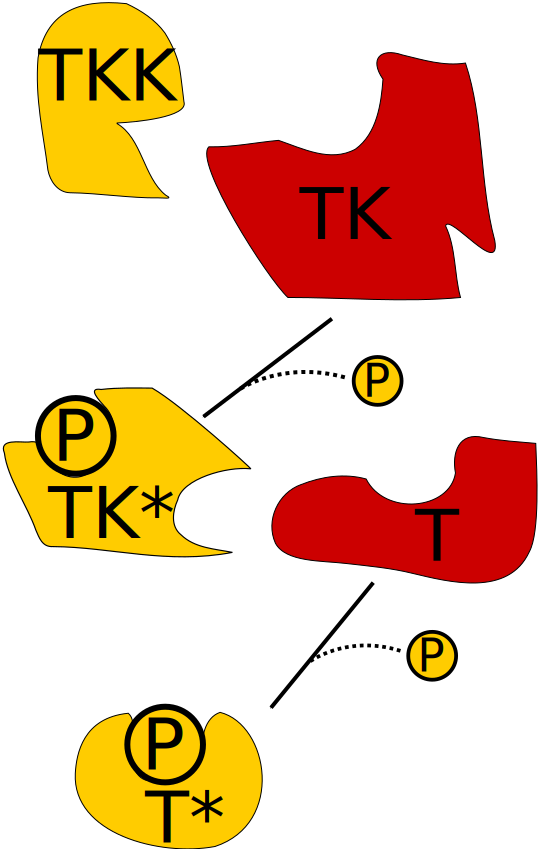
\includegraphics[width=.25\textwidth]{images/tkk_tk_t}}
%DIFDELCMD < \qquad%%%
\DIFdelendFL \DIFaddbeginFL \subfloat[\label{fig:small-example-net}]{\includegraphics[scale=\scalaRete]{images/tkk_tk_t_tutto_networkOnly}} \DIFaddendFL \qquad
\DIFaddbeginFL \subfloat[\label{fig:small-example01}]{\includegraphics[scale=\scalaRete]{images/tkk_tk_t_tutto01}} \DIFaddendFL \qquad
\DIFaddbeginFL \subfloat[\label{fig:small-example02}]{\includegraphics[scale=\scalaRete]{images/tkk_tk_t_tutto02}} \DIFaddendFL \qquad
\DIFdelbeginFL %DIFDELCMD < \subfloat[\label{fig:small-example-biology-network}]{
\includegraphics[width=.08\textwidth]{images/tkk_tk_t_network}}
%DIFDELCMD < %%%
\DIFdelendFL \DIFaddbeginFL \subfloat[\label{fig:small-example03}]{\includegraphics[scale=\scalaRete]{images/tkk_tk_t_tutto03}}
\DIFaddendFL \caption{...}\DIFaddbeginFL \label{fig:small-example-biology}
\DIFaddendFL \end{figure}

\DIFdelbegin %DIFDELCMD < \setlength{\abovecaptionskip}{2pt}
%DIFDELCMD < %%%
\DIFdelend %DIF >  \setlength{\abovecaptionskip}{2pt}

\DIFdelbegin \DIFdel{Experimental evidence shows }\DIFdelend \DIFaddbegin \DIFadd{The current knowledge on signaling pathways~\mbox{%DIFAUXCMD
\cite{kegg,phosphosite}
}%DIFAUXCMD
evidences the fact
}\DIFaddend that signaling interactions \DIFdelbegin \DIFdel{often }\DIFdelend \DIFaddbegin \DIFadd{are rarely a simple chain of activations as represented in Figure~\ref{fig:small-example-net}.
More often, they }\DIFaddend assume the shape of a network \DIFdelbegin \DIFdel{instead of a simple
chain of activations, with }\DIFdelend \DIFaddbegin \DIFadd{with multiple feedback loops and }\DIFaddend crosstalk from different signaling sources.
This \DIFdelbegin \DIFdel{complicates }\DIFdelend \DIFaddbegin \DIFadd{complexity is an added difficulty for }\DIFaddend the study of such networks, \DIFdelbegin \DIFdel{as
%DIF <  This makes the study of such networks a complex task, as
it is often difficult }\DIFdelend \DIFaddbegin \DIFadd{reducing the possibilities for the human brain alone
}\DIFaddend to deduce the dynamic behavior of a signaling network by inspecting its static representation.
For this reason, \DIFaddbegin \DIFadd{an efficient }\DIFaddend computational support is essential when representing and analyzing the behavior
of complex signaling networks.
%DIF <  The availability of computational models of such complex,
%DIF <  dynamic networks would allow the biologists to perform {\it in silico} experiments,
%DIF <  obtaining useful insights to help them plan new wet-lab experiments or formulate updated theories.
%DIF <  Moreover, traditional representations in the domain-specific language used for biological signaling networks
%DIF <  are often ambiguous, with extensive use of \emph{ad hoc} semantics, where
%DIF <  the same graphical elements acquire different meanings in different network representations.
%DIF <  While helping the understanding of the specific cases, this ambiguity makes it difficult to deal with various
%DIF <  representations at the same time, always requiring human intervention when integrating informations from multiple
%DIF <  sources into larger networks.


\subsection{\tas}\label{sec:TA}
\DIFdelbegin \DIFdel{\tas}%DIFDELCMD < \ %%%
\DIFdelend \DIFaddbegin \renewcommand{\ta}{TA}
\renewcommand{\tas}{TA}
\DIFadd{Timed Automata (\tas) }\DIFaddend are finite-state automata enriched with real-valued clocks
and synchronization channels. All clocks in a \tas\ system advance with the same rate,
and transitions between the locations of an automaton
depend on conditions on clocks. In particular, a \emph{guard} defines when a transition
may be taken, while an \emph{invariant} is the condition for permanence in a location.
A transition can also allow two automata to \emph{synchronize},
with each participant performing one of two complementary actions (\emph{input} and \emph{output})
on a \DIFdelbegin \DIFdel{communication }\DIFdelend \DIFaddbegin \DIFadd{synchronization }\DIFaddend channel. A set of clocks may also be reset by a transition, causing them to restart counting from 0.

\DIFdelbegin %DIFDELCMD < \begin{definition}[\ta]
%DIFDELCMD < %%%
%DIF <  Formal definition of T.A., which seems to be common practice among FORMATS papers
%DIFDELCMD < \ \\
%DIFDELCMD < %%%
\DIFdel{A \ta}%DIFDELCMD < \ %%%
\DIFdel{is a tuple $\langle{}L, l_0 , C, S, E, I\rangle$, where $L$ is a set of locations,
$l_0 \in L$ is the initial location, $C$ is the set of clocks, $S = A \times \{\mbox{\it input}, \mbox{\it output}\}$
is a set of synchronization channels (each containing an action label and identified as either }%DIFDELCMD < {\it %%%
\DIFdel{input}%DIFDELCMD < } %%%
\DIFdel{or }%DIFDELCMD < {\it %%%
\DIFdel{output}%DIFDELCMD < }%%%
\DIFdel{),
$E \subseteq L \times S \times {\cal B}(C) \times 2^C \times L$ is a set of transitions between locations with a synchronization channel,
a guard and a set of clocks to be reset, and $I : L \rightarrow {\cal B}(C)$ assigns invariants to locations.
}%DIFDELCMD < 

%DIFDELCMD < \end{definition}
%DIFDELCMD < %%%
\DIFdel{${\cal B}(C)$ is the set of boolean formulas defining bounds on clock values. For example, taken
$x, y \in C$, the expression $x \leq 10 \wedge y > 4$ is an element of ${\cal B}(C)$.
}%DIFDELCMD < 

%DIFDELCMD < %%%
\DIFdelend The models we will present here were implemented using the software tool UPPAAL~\cite{uppaal}, which adds a number of features
to the basic definition of \tas. Some of these extensions include: support for integer variables in addition to clocks,
broadcast \DIFdelbegin \DIFdel{communication }\DIFdelend \DIFaddbegin \DIFadd{synchronization }\DIFaddend channels (one sender, many receivers), definition of C-like functions to perform more 
operations \DIFdelbegin \DIFdel{other than }\DIFdelend \DIFaddbegin \DIFadd{besides }\DIFaddend clock resets.
UPPAAL also allows for a special type of locations, named \emph{committed} (marked with a {\sf C} in the graphical representation).
As long as an automaton is in a committed location, time is not allowed to flow. This feature can be used for example to perform immediate
updates to local variables before letting the computation proceed. %DIF < All such features will be considered as part of \tas\ for the rest of this paper.
\DIFdelbegin %DIFDELCMD < 

%DIFDELCMD < %%%
%DIF <  As an example of \tas\, we introduce in Figure~\ref{fig:small-example-model} a first basic model of a generic signalling network.
%DIF <  The model allows us to represent the active fraction (called from now on \emph{activity level}, or simply \emph{activity} when
%DIF <  not ambiguous) of a population of molecules as an integer variable ({\sf reactant}, Fig.~\ref{fig:small-example-model-reactant}),
%DIF <  whose value is changed by reactions with positive (Fig.~\ref{fig:small-example-model-activation}) or negative
%DIF <  (Fig.~\ref{fig:small-example-model-inhibition}) effect. In the example model, the value of {\sf reactant} is bounded
%DIF <  inside the interval $[0, \mbox{\sf MAX}]$, and reaching a bound is the only factor on which the decision to enable or disable a reaction
%DIF <  (locations {\sf Reacting}, {\sf NotReacting} in Figs.~\ref{fig:small-example-model-activation}, \ref{fig:small-example-model-inhibition})
%DIF <  is made. As we have explained in Section~\ref{sec:biologia} (Fig.~\ref{fig:small-example-biology-kinases}), a more precise model of a signalling
%DIF <  network should also allow to take into account the activity of upstream kinases when determining the availability of
%DIF <  an activating reaction.
%DIF <  
%DIF <  \def\taScalea{0.4}
%DIF <  \def\taScaleb{0.16}
%DIF <  
%DIF <  \begin{figure}[htb]
%DIF <  \centering
%DIF <  \subfloat[Reactant\label{fig:small-example-model-reactant}]{\includegraphics[scale=\taScaleb]{images/esempio_biologico_reactant}}\quad
%DIF <  \subfloat[Activation\label{fig:small-example-model-activation}]{\includegraphics[scale=\taScalea]{images/esempio_biologico_activation}}\quad
%DIF <  \subfloat[Inhibition\label{fig:small-example-model-inhibition}]{\includegraphics[scale=\taScalea]{images/esempio_biologico_inhibition}}
%DIF <  \caption{Three \tas\ templates to model a signalling pathway as represented by UPPAAL's user interface.
%DIF <  The automaton in {\protect\subref{fig:small-example-model-reactant}} updates the {\sf reactant} variable (with valid interval $[0, {\sf MAX}]$)
%DIF <  whenever a reaction occurs, changing its activity level.
%DIF <  {\protect\subref{fig:small-example-model-activation}} represents an activating reaction, which occurs when its internal clock {\sf c}
%DIF <  is inside the interval [{\sf LB, UB}], making the target reactant's activity level increase.
%DIF <  {\protect\subref{fig:small-example-model-inhibition}} represents an inhibition reaction, whose effect is the inverse
%DIF <  of activation.
%DIF <  Shared channels {\sf goUp} and {\sf goDown} are used for communication between reaction and reactant automata.
%DIF <  \label{fig:small-example-model}}
%DIF <  \end{figure}
%DIFDELCMD < 

%DIFDELCMD < %%%
%DIF <  \subsection{Biological signaling pathways}
%DIF <  %mostrare reti biologiche come si rappresentano tradizionalmente, per far vedere
%DIF <  %che con ANIMO si parte da quelle e le si estende mettendoci anche l'aspetto dinamico
%DIF <  %mostrare possibilmente anche grafici con picchi, di cui parliamo dopo (quando diciamo
%DIF <  %che ANIMO ti forza anche a considerare le disattivazioni, senno' il picco non lo ottieni mica)
%DIF <  A biological signaling pathway visually describes the network of interactions occurring
%DIF <  when a biological cell comes in contact with an external substance, as e.g. a drug.
%DIF <  When this happens, the signal is ``passed on'' between different molecules inside the cell,
%DIF <  \emph{activating} each other in turn, and possibly involving (positive or negative) feedback
%DIF <  mechanisms that allow to regulate the signaling process.
%DIF <  Figure~\ref{fig:pathway} shows an example pathway, based on the one shown in~\cite{pathway-autocrine},
%DIF <  where the \emph{crosstalk} between TNF (tumor necrosis factor), EGF (epidermal growth factor)
%DIF <  and insulin is represented: this highlights the complexity of the interactions happening
%DIF <  when one or multiple signals are received by a cell, showing how signal transduction paths with different origins interact with each other.
%DIF <  This manner of representing a pathway helps to understand which molecules are involved when
%DIF <  a particular input is received by a cell, but it is still difficult even for an expert biologist to properly understand which molecules
%DIF <  become activated, with how much strength and at which time from treatment. All these dynamic properties cannot be directly
%DIF <  deduced from the traditional, static pathway representations. Moreover, the semantics of the symbols used
%DIF <  such representations is often peculiar to a single representation, varying from case to
%DIF <  case. This may contribute in making a specific network more clear, but the absence of a formal
%DIF <  way of defining pathways hampers the integration of informations from multiple sources, which
%DIF <  often needs human intervention to be made homogeneous (see for example the databases~\cite{kegg,phosphosite},
%DIF <  which are largely manually curated).
%DIF <  
%DIF <  \begin{figure}[htbp]
%DIF <  \centering
%DIF <    \includegraphics[width=\textwidth]{images/pathway_riferimento_semplificato2}
%DIF <  \caption{A simplified representation of the pathways of TNF, EGF and insulin. $\rightarrow$
%DIF <  represents activation, while $\dashv$ stands for inhibition (i.e. inactivation). At each arrow
%DIF <  endpoint we find a different molecular species, but only those species whose activities were
%DIF <  measured in~\cite{pathway-compendium} have labels.
%DIF <  The part marked with {\sf Out} represents the outside of the cell,
%DIF <  while {\sf In} indicates the cytoplasm (inner side). \label{fig:pathway}}
%DIF <  \end{figure}
%DIF <  
%DIF <  
%DIF <  \subsection{\tas}
%DIF <  \tas\ are finite-state automata to which communication channels
%DIF <  and real-valued clocks have been added. In particular, clocks are used to define conditions enabling
%DIF <  certain transitions between the locations of an automaton, or to limit the permanence in a location. These conditions are called respectively
%DIF <  \emph{guards} and \emph{invariants}. Shared two-way and broadcast channels can be used to synchronize different automata.
%DIF <  Model checking can be performed on \tas\ models using the UPPAAL tool~\cite{uppaal},
%DIF <  thus obtaining answers to interesting questions about the correctness and behavior of models.
%DIF <  
%DIF <  In the example in Figure~\ref{fig:ta-example} (taken from~\cite{timed-automata}) we show two interacting \tas: a student~(Fig.~\ref{fig:ta-example-student})
%DIF <  and his table lamp~(Fig.~\ref{fig:ta-example-lamp}).
%DIF <  The starting locations (identified by a double circle, and labelled respectively {\sf idle} and {\sf off}) define the initial configuration for the system:
%DIF <  starting from that configuration, the model evolves following possibly different paths. In the example, from the {\sf idle}
%DIF <  location the student can move to {\sf relax} or {\sf study} after a non-deterministic choice, via respectively one and two synchronizations
%DIF <  with the lamp over the channel {\sf press}. Please notice that in order to reach the {\sf study} location (and thus let the lamp reach the {\sf bright} location)
%DIF <  the student needs to let no more than 10 time units elapse before performing the {\sf press} action a second time: the condition $\mbox{\sf y} < 5$,
%DIF <  which is even stricter than necessary, is used to this aim. Indeed, the lamp automaton imposes the guard $\mbox{\sf x} <= 10$ for the second consecutive
%DIF <  {\sf press?} action: if a communication on channel {\sf press} is not received after more than 10 time units have passed since the first
%DIF <  one was received, then the lamp goes automatically back to the {\sf off} location. It is interesting to notice that this model requires the student
%DIF <  to relax for at least 10 time units before reganining the {\sf idle} location: this is again due to the 10 time units limit
%DIF <  imposed by the lamp to transition from {\sf dim} to {\sf bright}.
%DIF <  
%DIF <  % Finally, please notice that the \emph{type} of a communication channel determines how the channel can be used: the channel of the example
%DIF <  % can be used for communication between exactly two participants, so if there are two lamps and the student sends a communication on the {\sf press}
%DIF <  % channel, only one will be able to react to it. If the channel was declared as \emph{broadcast}
%DIF <  % instead, any process able to receive a message on that channel would take part to the same communication: in that case,
%DIF <  % the student performing the {\sf press!} action with two lamps around would have made both lamps react.
%DIF <  
%DIF <  % \begin{figure}[htbp]
%DIF <  %   \centering
%DIF <  % \subfloat[]{
\includegraphics{images/esempio_uppaal_student}\label{fig:ta-example-student}}\qquad\qquad
%DIF <  % \subfloat[]{\includegraphics{images/esempio_uppaal_lamp}\label{fig:ta-example-lamp}}
%DIF <  % \caption{\tas\ models for the example: {\bf \subref{fig:ta-example-student}} the student, {\bf \subref{fig:ta-example-lamp}} the lamp.\label{fig:ta-example}}
%DIF <  % \end{figure}
\DIFdelend \DIFaddbegin \DIFadd{Examples of the listed features can be found in the
\tas}\ \DIFadd{model described in Section~\ref{sec:ta-model}.
}\DIFaddend 


\subsection{Activity-based models in ANIMO}\label{sec:animo-old}
\DIFdelbegin %DIFDELCMD < 

%DIFDELCMD < %%%
\DIFdelend ANIMO allows the definition of \emph{activity-based} models. This means that we assume each signaling molecule in a
cell to be at any time in one of two states: active or inactive. Active molecules can take an active role in reactions,
changing the state of other molecules, activating inactive molecules or inhibiting (i.e. \DIFdelbegin \DIFdel{de-activating}\DIFdelend \DIFaddbegin \DIFadd{deactivating}\DIFaddend ) active molecules.
In a kinase-based signaling network an activation process can be
a phosphorylation, and it is usually countered by the corresponding dephosphorylation. However, 
our models are not limited to kinase networks: other features like different post-translational
modifications or gene promotion can be likewise represented, as long as their role has immediate effects on the ability of a
target to perform its task.

A model in ANIMO is defined through the Cytoscape plug-in user interface (see Fig.~\ref{fig:cytoscape}), where the user inserts
a node for each molecular species and an \DIFdelbegin \DIFdel{arrow }\DIFdelend \DIFaddbegin \DIFadd{edge }\DIFaddend for each reaction, with $\rightarrow$ indicating activation
and $\dashv$ indicating inhibition similarly to traditional representations of signaling networks (\DIFdelbegin \DIFdel{see }\DIFdelend Fig.~\DIFdelbegin \DIFdel{\ref{fig:small-example-biology-network}).
%DIF <  The graphical representation of a network in ANIMO is based on traditional signaling network symbols (see Fig.~\ref{fig:small-example-biology-network}),
%DIF <  thus each node represents a molecular species, while arrows represent activating ($\rightarrow$) or inhibiting ($\dashv$) reactions.
}\DIFdelend \DIFaddbegin \DIFadd{\ref{fig:small-example-net}).
}

\begin{figure}[htb]
\begin{center}
   \includegraphics[width=.6\textwidth]{images/mapk_model_egf4}
\end{center}
\caption{...\label{fig:cytoscape}}
\end{figure}
\DIFaddend 

We consider a \emph{molecular species} (also called \emph{reactant}) to include all the molecules of the same substance in both their active
and inactive state inside the cell. In order to distinguish between the two activity states in which each molecule can be,
we define the \emph{activity level}
to represent the percentage of active molecules over an entire molecular species. In an ANIMO model, this value
is discretized on a given integer interval, to \DIFaddbegin \DIFadd{adapt to the quality
of available experimental data and (for large models) }\DIFaddend allow for a trade-off between performance and precision.
The user can choose the granularity for each molecular species separately, on a scale between 2 (the
reactant is seen as either completely inactive or completely active) and 101 levels (allowing to represent activity as $0, 1\%, 2\% \dots\ 100\%$).
\DIFdelbegin \DIFdel{This choice is made via the user interface as shown in Figure~\ref{fig:node-dialog}.
%DIF <  The graphical representation of a network in ANIMO is based on traditional signaling network symbols (see Fig.~\ref{fig:small-example-biology-network}),
%DIF <  thus each node represents a molecular species, while arrows represent activating ($\rightarrow$) or inhibiting ($\dashv$) reactions.
%DIF < The aim of our framework is the modeling of biological interaction networks, with a particular focus on signaling
%DIF < pathways.
%DIF <  In order to allow a biologist to operate in a familiar environment, ANIMO was implemented as a
%DIF <  Cytoscape~\cite{cytoscape} plug-in (see Fig.~\ref{fig:cytoscape}):
%DIF <  this allowed us to build an user interface based on an already existing and widely used biological tool,
%DIF <  opening further analysis possibilities thanks to the wide array of already existing plug-ins.
%DIF <  
%DIF <  
%DIF <  Users are presented with an interface allowing them to define the topology of a pathway in the traditional way: thus, each interacting
%DIF <  molecular species is represented by a node (e.g., node {\sf MK2} represents the entire population of molecules of type MK2 inside the cell),
%DIF <  while edges represent activating or inhibiting influences.
%DIF <  We call the models defined in ANIMO \emph{activity-based}. With this we mean that model molecular interactions are modelled
%DIF <  in terms of variation of activity, where a single molecule is assumed to have only two states, active and inactive.
}\DIFdelend The activity level of a molecular species is represented in the ANIMO network
by coloring the corresponding node according to the scale shown in the {\sf Activity} legend in Figure~\ref{fig:cytoscape},
where the minimum indicates that all molecules of the given species are inactive.
%DIF <  As our model represents
%DIF <  the activity level of a reactant with an integer variable, the user interface allows to choose the number of discrete
%DIF <  levels that represent that activity level, ranging on a scale between 2 and 100 (cf. Fig.~\ref{fig:node-dialog}).
%DIF <  This allows the user to choose a different granularity for each node of the network, allowing for higher precision
%DIF <  where there is more confidence, and approaching a Boolean style of modeling where only a generic behavior is wanted.
\DIFdelbegin %DIFDELCMD < 

%DIFDELCMD < \def\mygraphic{\includegraphics[scale=.35]{images/cytoscape_edge_dialog5}}
%DIFDELCMD < \newlength\graphicheight
%DIFDELCMD < \setlength\graphicheight{\heightof{\mygraphic}}
%DIFDELCMD < \begin{figure}[htbp]
%DIFDELCMD < \begin{center}
%DIFDELCMD <    \subfloat[]{\includegraphics[width=.9\textwidth]{images/mapk_model_egf4}\label{fig:cytoscape}}\\
%DIFDELCMD <    \subfloat[]{\begin{minipage}[c][\graphicheight]{0.45\textwidth}\begin{center}\includegraphics[scale=.35]{images/cytoscape_node_dialog3}\end{center}\end{minipage}\label{fig:node-dialog}}
%DIFDELCMD <    \quad\subfloat[]{\begin{minipage}[c][\graphicheight]{0.45\textwidth}\begin{center}\mygraphic\end{center}\end{minipage}\label{fig:edge-dialog}}
%DIFDELCMD < \end{center}
%DIFDELCMD < %%%
%DIFDELCMD < \caption{%
{%DIFAUXCMD
%DIFDELCMD < {\bf \protect\subref{fig:cytoscape}} %%%
\DIFdel{The Cytoscape user interface running the ANIMO plug-in
(image from~\mbox{%DIFAUXCMD
\cite{animo-bibe}
}%DIFAUXCMD
). The }\emph{\DIFdel{Network}} %DIFAUXCMD
\DIFdel{panel in the center contains the nodes-arrows
model of the crosstalking signaling pathways of NGF and EGF, with
colors indicating node activity levels and shapes representing different protein categories (see the }\emph{\DIFdel{Legend}} %DIFAUXCMD
\DIFdel{on the left).
The }\emph{\DIFdel{Results Panel}} %DIFAUXCMD
\DIFdel{on the right contains a graph plotting activity levels of selected nodes
during the first hour of evolution of the model. The slider under the graph
allows the user to select the time instant (marked as a vertical red line in the graph) on which
the colors nodes in the }\emph{\DIFdel{Network}} %DIFAUXCMD
\DIFdel{are based.
%DIF <  The series with the {\sf \_data} suffix is experimental
%DIF <  data from~\cite{egf-ngf}, considering a treatment with 100~ng/ml EGF.
}%DIFDELCMD < {\bf \protect\subref{fig:node-dialog}} %%%
\DIFdel{The }\emph{\DIFdel{Edit reactant}} %DIFAUXCMD
\DIFdel{dialog: it is possible to
assign to each reactant a name, molecule type (changing how the node is displayed to the user),
granularity and initial activity level.
%DIF <  whether the reactant is enabled and whether it will be shown in a simulation run plot.
%DIF <  Only enabled reactants are taken into account when analyzing the network, and only reactants marked as \emph{Plotted}
%DIF <  are plotted in a graph representing a simulation run.
}%DIFDELCMD < {\bf \protect\subref{fig:edge-dialog}} %%%
\DIFdel{The }\emph{\DIFdel{Edit reaction}} %DIFAUXCMD
\DIFdel{dialog:
the user chooses a kinetic scenario, sets a value for
the kinetic constant $k$ (either quantitative or qualitative), 
and defines whether the reaction is activating or inhibiting.}%DIFDELCMD < \label{fig:cytoscape-ui}%%%
}
%DIFAUXCMD
%DIFDELCMD < \end{figure}
%DIFDELCMD < %%%
\DIFdelend 

The occurrence of a \emph{reaction} modifies by one discrete step the activity level of its target reactant, making it increase or decrease 
depending on whether the reaction is defined, respectively, as activating or inhibiting.
The rate with which a reaction occurs depends on a formula selected by the user\DIFdelbegin \DIFdel{via the dialog represented in Figure~\ref{fig:edge-dialog}}\DIFdelend . 
Choosing one of \DIFdelbegin \DIFdel{the }\DIFdelend three available scenarios allows the user to make the reaction rate depend on
the activity of one or two reactants.
%DIF <  The first scenario depends only on the activity level of the upstream reactant:
%DIF <  the more that reactant is active, the faster the reaction will proceed.
%DIF <  The second scenario depends on both participating reactants: it is directly correlated to the activity level of 
%DIF <  the upstream reactant, and inversely (resp. directly) correlated to the activity of the downstream one if the
%DIF <  reaction has activating (resp. inhibiting) influence. The third scenario depends on two reactants, none of which
%DIF <  needs to be the downstream one: this scenario is useful to represent the so-called \emph{AND port}, which requires
%DIF <  two reactants to be both active at the same time in order to activate a third one. An AND port can be used e.g.
%DIF <  as a rough representation of complexation, where two molecules join together to form a third molecule with a different function,
%DIF <  or to abstract a sub-network of complex interactions into a single reaction.
The rate of each reaction can be scaled by modifying the value of \DIFdelbegin \DIFdel{the }\DIFdelend \DIFaddbegin \DIFadd{one }\DIFaddend kinetic constant $k$,
possibly using a qualitative measure from a predefined set ({\sf very slow}, {\sf slow},
{\sf medium}, {\sf fast}, {\sf very fast}\DIFdelbegin \DIFdel{, see Fig.~\ref{fig:edge-dialog}}\DIFdelend ).
Approximating the actual reaction dynamics with less detailed single-parameter scenarios
leads to a kinetic model that is still precise enough to faithfully represent the behavior of a signaling network.
%DIF <  This can come especially useful when building a
%DIF <  new model: in order to define the topology of the pathway, only qualitative parameters can be chosen for reactions, 
%DIF <  while the user concentrates on obtaining the correct order of reactant activity peaks. As a next step, the model 
%DIF <  can be more precisely defined by manually tweaking the scenario parameters, and thus better fit the available experimental data.
%DIF <  
%DIF <  During the modeling process, the user can inspect the time evolution of the system by
%DIF <  pressing the \emph{Analyze network} button.
%DIF <  Automatically, an \tas\ model is generated and simulation data series
%DIF <  are obtained thanks to UPPAAL. The results are then parsed and presented as a graph plotting
%DIF <  the activity level of selected reactants over the desired time interval.
%DIF <  Interacting with the slider under the graph lets the user observe the evolution of the
%DIF <  network along the simulation interval, with the activity levels of all nodes mirrored as colors
%DIF <  in the \emph{Network} panel (see Fig.~\ref{fig:cytoscape}).
%DIF <  This feature helps to better understand which signals are active at any given instant, and thus decide whether the model 
%DIF <  behaves as expected. When unexpected behavior is found, there arises the possibility to generate new hypotheses or decide
%DIF <  which direction the next laboratory experiments should take.
%DIF < 
%DIF <  It is also possible to temporarily disable (groups of) reactions or reactants in the graph: this allows the user to
%DIF <  concentrate the modeling effort to a specific part of the network, or to test what the knock-out of a reactant would
%DIF <  cause to the behavior of the system. This is an example of an \emph{in silico} experiment, which can be of great help to the biologist, making it
%DIF <  easier to understand and extend the existing knowledge on signaling pathways.
%DIF < 
%DIF <  An example consequence of this approach is that in order to obtain the typical peak dynamics shown by experimental
%DIF <  data the user needs to consider both activating and inhibiting reactions, thus forcing a more objective point of view
%DIF <  than the traditional one, where only activations are often considered.
%DIF < 
\DIFaddbegin \DIFadd{The approximation allows us to reduce the dependence of a model from often unavailable quantitative
parameters for biochemical reaction kinetics.
}\DIFaddend For a more precise dissertation on how reaction rates are computed in ANIMO, we \DIFdelbegin \DIFdel{refer the interested reader to~\mbox{%DIFAUXCMD
\cite{animo-bibe}
}%DIFAUXCMD
}\DIFdelend \DIFaddbegin \DIFadd{recommend~\mbox{%DIFAUXCMD
\cite{animo-ieee}
}%DIFAUXCMD
}\DIFaddend ,
where the \DIFdelbegin \DIFdel{currently }\DIFdelend \DIFaddbegin \DIFadd{previously }\DIFaddend used \tas\ model is presented. \DIFdelbegin %DIFDELCMD < 

%DIFDELCMD < %%%
%DIF <  \begin{figure}[htbp]
%DIF <  \centering
%DIF <    \subfloat[]{\includegraphics[scale=.37]{images/cytoscape_node_dialog2}\label{fig:node-dialog}}
%DIF <  %   \subfigure[Dialog for reaction
%DIF <  % properties.]{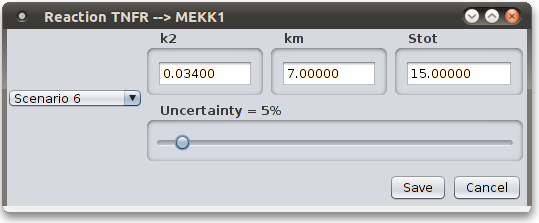
\includegraphics[scale=.45]{images/cytoscape_edge_dialog}\label{fig:edge-dialog}}
%DIF <  \quad
%DIF <    \subfloat[]{\includegraphics[scale=.37]{images/cytoscape_edge_dialog4}\label{fig:edge-dialog}}%2}}
%DIF <  \caption{Setting the properties for reactants and reactions. {\bf \protect\subref{fig:node-dialog}} The \emph{reactant}
%DIF <  dialog: it is possible to
%DIF <  choose the name to be displayed on the node representing the reactant, 
%DIF <  the type of molecule (changing how the node is displayed to the user)
%DIF <  the available number of activity levels (i.e., the granularity),
%DIF <  the initial level of activity,
%DIF <  whether the reactant is enabled and whether it will be shown in a simulation run plot.
%DIF <  Only enabled reactants are taken into account when analyzing the network, and only reactants marked as \emph{Plotted}
%DIF <  are plotted in a graph representing a simulation run. {\bf \protect\subref{fig:edge-dialog}} The \emph{reaction} dialog:
%DIF <  it is possible to choose the kinetic approximation scenario, set a value for
%DIF <  the kinetic constant $k$ (either quantitative or qualitative), 
%DIF <  and define the influence of the reaction, where \emph{Activation} means positive
%DIF <  and \emph{Inhibition} negative.
%DIF <  \label{fig:cytoscape-dialogs}}
%DIF <  \end{figure}
\DIFdelend \DIFaddbegin \DIFadd{The reader interested in the current
methods for parameter setting in ANIMO can refer to~\mbox{%DIFAUXCMD
\cite{animo-syncop}
}%DIFAUXCMD
.
}\DIFaddend 




\section{A new way of modeling signaling pathways \DIFdelbegin %DIFDELCMD < \\%%%
\DIFdelend with \tas}\label{sec:animo-new}
We propose here a novel \DIFdelbegin \DIFdel{\tas}%DIFDELCMD < \ %%%
\DIFdelend model to represent signaling pathways \DIFdelbegin \DIFdel{.
%DIF <  As we will show, this model is in general more efficient both in terms of computation
%DIF <  time and memory usage with respect to the model presented in~\cite{animo-bibe}.
}\DIFdelend \DIFaddbegin \DIFadd{with \tas.
}\DIFaddend We define the model \DIFdelbegin \DIFdel{currently }\DIFdelend \DIFaddbegin \DIFadd{previously }\DIFaddend used in ANIMO to be \emph{reaction-centered}, as for each reaction
in the network an instance of a \ta\ template is generated to \DIFdelbegin \DIFdel{mimick
}\DIFdelend \DIFaddbegin \DIFadd{mimic
}\DIFaddend the occurrences of that reaction\DIFdelbegin \DIFdel{, whose dynamics depend on its upstream reactant(s) and
whose influence changes the activity level of its downstream reactant}\DIFdelend . Observing that signaling
networks tend to be highly connected, containing noticeably more reactions than reactants,
we propose to shift the focus on reactants instead, achieving \DIFaddbegin \DIFadd{what we call }\DIFaddend a \emph{reactant-centered} model.
%DIF < Figure~\ref{fig:ta-new-model} shows the template at the base of the proposed model.
\DIFaddbegin \DIFadd{This change of view is inspired by the classical way in which biological events are modeled
with ordinary differential equations (ODEs)~\mbox{%DIFAUXCMD
\cite{ode-ma-anche-altro}
}%DIFAUXCMD
.
}\DIFaddend 

\DIFdelbegin %DIFDELCMD < \begin{figure}[htb]
%DIFDELCMD <   %%%
\DIFdelend %DIF >  \begin{figure}
%DIF >    \centering
%DIF >    \includegraphics[width=0.3\textwidth]{images/network_abcd}
%DIF >  \caption{A signaling network where one node is influenced by three distinct reactions.
%DIF >  The (virtual) reaction $R_A$ is defined in the reactant-centered model
%DIF >  as the algebraic sum of the reactions influencing $A$.
%DIF >  % The reaction-centered ANIMO model from~\cite{animo-ieee} would generate three
%DIF >  % \tas, while the model presented here would lead a single automaton representing $R_A$.
%DIF >  }\label{fig:network-abcd}
%DIF >  \end{figure}
\DIFaddbegin 


\def\scalaOldModel{0.25}
\def\reactantTA{\includegraphics[scale=0.35]{images/Reactant_R3}}
\newlength\reactantTAheight
\setlength\reactantTAheight{\heightof{\reactantTA}}

\begin{figure*}[!htb]
  \DIFaddendFL \begin{center}
  \DIFdelbeginFL %DIFDELCMD < \includegraphics[width=\textwidth]{images/Reactant_R3}
%DIFDELCMD <   %%%
\DIFdelendFL \DIFaddbeginFL \subfloat[\label{fig:network-abcd}]{\begin{minipage}[c][\reactantTAheight]{0.18\textwidth}\begin{center}\includegraphics[scale=1.0]{images/network_abcd}\end{center}\end{minipage}} \qquad\qquad
  \subfloat[$R_A$\label{fig:ta-new-model}]{\begin{minipage}[c][\reactantTAheight]{0.6\textwidth}\begin{center}\reactantTA\end{center}\end{minipage}} \\
  \subfloat[$R_1: B \rightarrow A$ \label{fig:ta-old-BA}]{\includegraphics[scale=\scalaOldModel]{images/Reaction_B_A}} \qquad\qquad
%DIF >    \subfloat[$R_2: C \rightarrow A$ \label{fig:ta-old-CA}]{\includegraphics[scale=\scalaOldModel]{images/Reaction_C_A}} \qquad\qquad
  \subfloat[$R_3: D \dashv A$ \label{fig:ta-old-DA}]{\includegraphics[scale=\scalaOldModel]{images/Reaction_D_A}}
  \DIFaddendFL \end{center}
  \caption{...\label{fig:ta-models}}
\DIFdelbeginFL %DIFDELCMD < \end{figure}
%DIFDELCMD < %%%
\DIFdelendFL \DIFaddbeginFL \end{figure*}
\DIFaddend 

\DIFaddbegin \subsection{\DIFadd{Reactant-centered model}}\label{sec:reactant-centered}
\DIFaddend The reactant-centered model presented here is based on the concept of \emph{net effect} of a set of reactions on a reactant:
instead of considering each reaction in isolation, we consider their combined influence on each reactant.
%DIF < The idea at the base of the model is to sum the effects of all reactions influencing a reactant.
As an example, consider a reactant $A$ activated by reactions $R_1$ and $R_2$, and inhibited
by reaction $R_3$ \DIFaddbegin \DIFadd{(see Fig.~\ref{fig:network-abcd})}\DIFaddend .
The net effect of these three reactions on $A$ defines the \emph{net reaction} $R_A = R_1 + R_2 - R_3.$
Applying a concept similar to the definition of an \DIFdelbegin \DIFdel{ordinary differential equation}\DIFdelend \DIFaddbegin \DIFadd{ODE}\DIFaddend ,
where the rate of change of each reactant depends on the rate of the reactions influencing it,
the rate of $R_A$ is computed as the sum of the rates of the reactions influencing~$A$: 
$$r_A = r_1 + r_2 - r_3$$
where $r_i$ is the rate of reaction $R_i$ and is defined as follows.
Consider $R_1$ to be \DIFdelbegin \DIFdel{defined as }\DIFdelend \DIFaddbegin \DIFadd{the reaction }\DIFaddend $B \rightarrow A$ with kinetic constant $k_1$.
Suppose the settings \DIFaddbegin \DIFadd{in the ANIMO network }\DIFaddend for $R_1$ make its rate depend \DIFaddbegin \DIFadd{only }\DIFaddend on the
activity level of $B$. Then we compute the rate of $R_1$ as \DIFdelbegin \DIFdel{$r_1 = B \times k_1$}\DIFdelend \DIFaddbegin \DIFadd{$r_1 = [B] \times k_1$, with
$[B]$ the current activity level of $B$}\DIFaddend .



As with ODEs, if $r_A$ is positive the activity level of $A$ will increase;
otherwise, $A$ will decrease its activity level.
The absolute value of $r_A$ determines the speed with which such change happens.
The value of the reaction rate is \DIFdelbegin \DIFdel{then }\DIFdelend \DIFaddbegin \DIFadd{thus }\DIFaddend translated into a time value to be used as
time bound in the \ta\ representing $R_A$ (see Fig.~\ref{fig:ta-new-model}) by computing
$$T_A = \frac{1}{\mbox{abs}(r_a)}$$
with $\mbox{abs}(r_a)$ the absolute value of $r_a$. \DIFdelbegin %DIFDELCMD < \\
%DIFDELCMD < %%%
\DIFdelend \DIFaddbegin \DIFadd{In order to represent
a natural variability in reaction timing, we relax the exact value of $T_A$ by
defining bounds of~$\pm~5\%$:
}$$\DIFadd{
\begin{array}{lcl}
  \mbox{\sf tL} &=& T_A \times 0.95 \\
  \mbox{\sf tU} &=& T_A \times 1.05
\end{array}
}$$
\DIFadd{Analogously to the reaction-centered model of~\mbox{%DIFAUXCMD
\cite{animo-ieee}
}%DIFAUXCMD
,
we will call }{\sf \DIFadd{tL}} \DIFadd{the }\emph{\DIFadd{lower time bound}} \DIFadd{and }{\sf \DIFadd{tU}} \DIFadd{the }\emph{\DIFadd{upper time bound}}\DIFadd{.
Note that here, differently from what presented in~\mbox{%DIFAUXCMD
\cite{animo-ieee}
}%DIFAUXCMD
, we do not define
pre-computed tables with all possible values for }{\sf \DIFadd{tL}} \DIFadd{and }{\sf \DIFadd{tU}}\DIFadd{: this is because
the number of variables for the computation of a reaction rate can be arbitrarily high, and
the size of such tables grows exponentially with the number of variables.
In the example of Figure~\ref{fig:ta-models}, a table to represent the time bounds
for reaction ${R_A}$ would have four dimensions, depending on the activity levels
of reactants $A$, $B$, $C$ and $D$. Assuming that all four reactants are discretized
on 101 levels, each of the two tables }{\sf \DIFadd{tL}} \DIFadd{and }{\sf \DIFadd{tU}} \DIFadd{would contain $101^4 = 104\,060\,401$
elements. Adding one other reaction $E \rightarrow A$ to the pool would make
this approach exceed the memory limits of most of the currently available computers, requiring about 78 gigabytes of memory
to be stored. For this reason, the reaction rates are computed on the fly (see Section~\ref{sec:rates-ta-model}).
}


\subsection{\DIFadd{\tas}\ \DIFadd{model}}\label{sec:ta-model}
\DIFaddend The behavior of the \ta\ representing the net reaction $R_A$ is defined as follows: after \DIFdelbegin \DIFdel{$T_A$ seconds
}\DIFdelend \DIFaddbegin \DIFadd{a number of seconds
variable inside the continuous interval $[\mbox{\sf tL}, \mbox{\sf tU}]$ }\DIFaddend (measured with the local clock {\sf c}),
the activity level of $A$ will increase or
decrease by one step, depending on the sign of $r_A$; then \DIFdelbegin \DIFdel{a new value }\DIFdelend \DIFaddbegin \DIFadd{new values }\DIFaddend for $r_A$\DIFdelbegin \DIFdel{and $T_A$ }\DIFdelend \DIFaddbegin \DIFadd{, }{\sf \DIFadd{tL}} \DIFadd{and }{\sf \DIFadd{tU}} \DIFaddend will be computed based
on the (possibly) changed conditions.

The process described \DIFdelbegin \DIFdel{above }\DIFdelend \DIFaddbegin \DIFadd{in Section~\ref{sec:reactant-centered} }\DIFaddend to compute the \DIFdelbegin \DIFdel{value of $T_A$ }\DIFdelend \DIFaddbegin \DIFadd{values of }{\sf \DIFadd{tL}} \DIFadd{and }{\sf \DIFadd{tU}} \DIFaddend is an instance of the function called {\sf update()}
in the \ta\ template of Figure~\ref{fig:ta-new-model}\DIFdelbegin \DIFdel{(where $T_A$ is called }%DIFDELCMD < {\sf %%%
\DIFdel{T}%DIFDELCMD < }%%%
\DIFdel{)}\DIFdelend . The computation of {\sf update()} is the first step
taken when initializing a new model taking the transition from the initial location {\sf start} (identified by two concentric circles)
to {\sf updating}.
Location {\sf updating} is then used to decide whether $R_A$ can be executed or not (functions
{\sf can\_react()} and {\sf cant\_react()} used as guards for the transitions exiting from {\sf updating}).
This decision is based on the computed value for
$r_A$ and the current activity level of $A$: if $r_A > 0$ and $A$ is already completely active
(or  $r_A < 0$ and $A$ is completely inactive), no
update to $A$ can be applied, so the automaton switches to location {\sf not\_reacting}.
Moreover, $r_A$ can be $0$: this means
that the reactions influencing $A$ balance each other to complete cancellation, so also in this
case $R_A$ cannot occur and the next location will be {\sf not\_reacting}. Otherwise (i.e. if {\sf can\_react()} is true), the activity
level of $A$ can be changed, so the next location will be the one labeled {\sf waiting}, which
is reached after having made sure that its clock invariant is respected (committed location
between {\sf updating} and {\sf waiting}).

When in location {\sf waiting}, the local clock {\sf c}
is let run until \DIFdelbegin \DIFdel{the time required }\DIFdelend \DIFaddbegin \DIFadd{enough time has passed }\DIFaddend for the reaction to occur\DIFdelbegin \DIFdel{is reached}\DIFdelend : this is obtained by using {\sf c \DIFdelbegin \DIFdel{$<=$ T}\DIFdelend \DIFaddbegin \DIFadd{$>=$ tL}\DIFaddend } as \DIFdelbegin \DIFdel{invariant for location }\DIFdelend \DIFaddbegin \DIFadd{guard
for the transition from }\DIFaddend {\sf waiting} \DIFaddbegin \DIFadd{to }{\sf \DIFadd{updating}}\DIFaddend .
Because of \DIFdelbegin \DIFdel{this invariant, the transition from }\DIFdelend \DIFaddbegin \DIFadd{the invariant }{\sf \DIFadd{c $<=$ tU}} \DIFadd{on }\DIFaddend {\sf waiting}\DIFdelbegin \DIFdel{to }\DIFdelend \DIFaddbegin \DIFadd{, we ensure that the reaction occurs after no more than }\DIFaddend {\sf \DIFdelbegin \DIFdel{updating}\DIFdelend \DIFaddbegin \DIFadd{tU}\DIFaddend } \DIFdelbegin \DIFdel{is taken as soon as its guard }\DIFdelend \DIFaddbegin \DIFadd{seconds have passed.
The transition to }\DIFaddend {\sf \DIFdelbegin \DIFdel{c $>=$ T}\DIFdelend \DIFaddbegin \DIFadd{updating}\DIFaddend } \DIFdelbegin \DIFdel{holds,
leading }\DIFdelend \DIFaddbegin \DIFadd{leads }\DIFaddend to an update to the activity level of $A$ (call to {\sf react()}), together with the computation of new values for $r_A$\DIFdelbegin \DIFdel{and
$T_A$ }\DIFdelend \DIFaddbegin \DIFadd{,
}{\sf \DIFadd{tL}} \DIFadd{and }{\sf \DIFadd{tU}} \DIFaddend (function {\sf react()} calls {\sf update()}). Moreover, we see in Figure~\ref{fig:ta-new-model}
that a communication is sent on channel {\sf reacting[0]} ($0$ is the index
assigned to reactant $A$): this is used to warn
%DIF <  the automata representing reactants influenced by reactions depending on the activity level
%DIF <  of $A$ that such activity level has just changed, possibly changing the conditions for those reactions.
the other automata that the activity level of $A$ has just changed, possibly changing the conditions for
other reactions.

On the other hand, one of the reactants influencing a reaction on which $A$ depends may change its activity level
before $R_A$ can occur: this event may have an influence on the value of $r_A$, so a re-computation
of $r_A$\DIFdelbegin \DIFdel{and $T_A$ }\DIFdelend \DIFaddbegin \DIFadd{, }{\sf \DIFadd{tL}} \DIFadd{and }{\sf \DIFadd{tU}} \DIFaddend is needed.
In the template of Figure~\ref{fig:ta-new-model}, the indexes of the influencing reactants are 1, 2 and \DIFdelbegin \DIFdel{3.
}\DIFdelend \DIFaddbegin \DIFadd{3,
corresponding respectively to $B$, $C$, $D$ in Figure~\ref{fig:network-abcd}.
}\DIFaddend Whenever a communication on one of the channels corresponding to an influencing
reactant is received while in location {\sf waiting}, the automaton moves to location
{\sf stubborn}. This location was introduced to avoid unwanted non-deterministic behavior\DIFaddbegin \footnote{\DIFadd{The term }\emph{\DIFadd{unwanted}}
\DIFadd{refers to a non-determinism that is not related to actual biological concepts, but to the semantics of the modeling
paradigm.}} \DIFaddend in the model.
In the example, this could happen when the activity level of $B$ is updated concurrently (in the same instant) with the activity level of $A$.
As $B$ influences $A$ through reaction $R_1$, any change in the activity level of $B$ causes a change in $r_1$, thus
requiring a recomputation of $r_A$\DIFdelbegin \DIFdel{and $T_A$}\DIFdelend \DIFaddbegin \DIFadd{, }{\sf \DIFadd{tL}} \DIFadd{and }{\sf \DIFadd{tU}}\DIFaddend . Due to the interleaving nature of \tas\ semantics, only one automaton
may change location for the \tas\ system to change state. This means that, should the activity level of $B$ be changed
first, the conditions for $R_A$ would be recomputed, possibly preventing the update to $A$ to occur. Vice versa, should the activity
level of $A$ be changed first, both $A$ and $B$ could change their activity levels.
%DIF <  Such non-determinism can be caused by two or more reactants changing their activity level at the same instant:
%DIF <  in that case, the (non-deterministic) order in which the updates are computed could decide the behavior of the model.
In such a situation, the non-deterministic order in which the updates are computed decides the behavior of the model.
To avoid this, we ensure that if a reaction can occur in a given instant (i.e. {\sf c \DIFdelbegin \DIFdel{$=$ T}\DIFdelend \DIFaddbegin \DIFadd{$>=$ tL}\DIFaddend }), it will \DIFdelbegin \DIFdel{occur without
considering }\DIFdelend \DIFaddbegin \DIFadd{not
consider }\DIFaddend the concurrent updates to influencing reactants (in the example, \DIFdelbegin \DIFdel{$R_A$ would always occur when }\DIFdelend \DIFaddbegin \DIFadd{having the clock reach }\DIFaddend {\sf \DIFdelbegin \DIFdel{c $=$ T}\DIFdelend \DIFaddbegin \DIFadd{tL}\DIFaddend } \DIFaddbegin \DIFadd{ensures that $R_A$ occurs}\DIFaddend ,
independently from any concurrent update to $B$).
Performing a check on the current value of the clock {\sf c} with respect to the reaction \DIFdelbegin \DIFdel{time limit }\DIFdelend \DIFaddbegin \DIFadd{lower time bound }\DIFaddend allows
an automaton to detect the case of a concurrent update, remaining ``stubborn'' in its resolution
of reacting with the current configuration: the guard {\sf c $>=$ \DIFdelbegin \DIFdel{T}\DIFdelend \DIFaddbegin \DIFadd{tL}\DIFaddend } on
the transition returning from {\sf stubborn} to {\sf waiting}
%DIF < together with the invariant {\sf c $<=$ T} on {\sf waiting}
is the same as the guard on the transition from {\sf waiting} to {\sf updating} and
%DIF < ensures that no time will pass before the reaction will take place.
\DIFdelbegin \DIFdel{ensures that the reaction will }\DIFdelend \DIFaddbegin \DIFadd{implies that the transition could }\DIFaddend occur in the \DIFdelbegin \DIFdel{same }\DIFdelend \DIFaddbegin \DIFadd{current }\DIFaddend time instant.
If no conflict is found, i.e. {\sf c $<$ \DIFdelbegin \DIFdel{T}\DIFdelend \DIFaddbegin \DIFadd{tL}\DIFaddend }, a new time limit for the reaction is
computed via function {\sf update()} while moving to location {\sf updating}. Note that the clock {\sf c} is not reset
when moving from {\sf stubborn} to {\sf updating}: should the new conditions only change the value of {\sf \DIFdelbegin \DIFdel{T}\DIFdelend \DIFaddbegin \DIFadd{tL}} \DIFadd{and }{\sf \DIFadd{tU}\DIFaddend }
without disabling the reaction, the ``partial work'' of the reactions is not discarded.

Finally, location {\sf not\_reacting} is used to avoid reacting when not necessary (see the description
of {\sf cant\_react()} above), and to respond to changes in those reactants
which can influence the value of $r_A$. Should one of such reactants change its activity level, the
conditions are updated and the local clock is reset, moving to {\sf updating} to check whether the reaction can now
occur.

\DIFaddbegin \subsection{\DIFadd{Computations on the fly}}\label{sec:rates-ta-model}
\DIFaddend Reaction rates are all computed at run-time by function {\sf update()},
and are based on the user-chosen scenarios, their kinetic constant $k$ and the activity level of the involved reactants.
As such computations require floating-point precision but UPPAAL only provides integer
variables and operators, we use a significand-and-exponent notation with 4 significant figures, which allows for an error
in the order of $0.1 \%$ while 
avoiding integer overflow in UPPAAL's engine. As an example of such a notation, consider the two floating-point numbers
$a = 1.23456$ and $b = 0.00023456$, and their sum $c = a + b = 1.23479456$. The corresponding representations in
our integer-based notation will be:
$$\DIFdelbegin \DIFdel{
\begin{array}{r@{\hskip 4mm}r@{\hskip 4mm}c@{\hskip 4mm}rcl}
  \mbox{significand}(a) = 1235 & \mbox{exponent}(a) = -3 & \rightarrow & a &=& 1235 \times 10^{-3}\\
  \mbox{significand}(b) = 2346 & \mbox{exponent}(b) = -7 & \rightarrow & b &=& 2346 \times 10^{-7}\\
  \mbox{significand}(a + b) = 1237 & \mbox{exponent}(a + b) = -3 & \rightarrow & a+b &=& 1237 \times 10^{-3}
\end{array}
}\DIFdelend \DIFaddbegin \DIFadd{
\begin{array}{rcl}
  a = \langle 1235, -3 \rangle &=& 1235 \times 10^{-3}\\
  b = \langle 2346, -7 \rangle &=& 2346 \times 10^{-7}\\
  a + b = \langle 1237, -3 \rangle &=& 1237 \times 10^{-3}
\end{array}
}\DIFaddend $$
In this case, the number representing the sum $a + b$ differs from the exact result by $c - 1237 \times 10^{-3} = 0.001456$.
The interested reader can find the UPPAAL definitions and functions needed to compute rate and time values for the \tas\ templates
\DIFdelbegin \DIFdel{in Appendix~\ref{apx:double-functions} or }\DIFdelend %DIF >  in Appendix~\ref{apx:double-functions} or 
inside any UPPAAL model file generated by ANIMO with a reactant-centered model type.


\DIFaddbegin \subsection{\DIFadd{Comparison with previous \tas}\ \DIFadd{model}}\label{sec:ta-notes}
%DIF >  A qualitative parallel between the reactant- and reaction-centered versions of the \tas\ model
%DIF >  can be made by intuitively matching locations with the same name on the two models.
\DIFadd{With reference to Figures~\ref{fig:ta-new-model} and~\ref{fig:ta-models}{\protect\subref*{fig:ta-old-BA}\--{}\protect\subref*{fig:ta-old-DA}},
we propose a qualitative parallel between the reaction- (old) and reactant-centered (new) \tas}\ \DIFadd{models.
The first remark is that equally-named locations have the same function in the automaton: so for
example location }{\sf \DIFadd{waiting}} \DIFadd{is used to wait before updating the reactant.
The central location is in both cases labelled }{\sf \DIFadd{waiting}}\DIFadd{: there the automaton waits
until the time has come for the reaction to occur. The amount of time to be waited has different meanings:
in the reaction-centered model, 
}

\DIFadd{Being based on the same abstractions, the queries the two models can be analyzed with the same
UPPAAL queries for all the cases for which biology is involved. The differences can be seen only if the
analysis focuses on the single automaton level and explicitly refers to locations: such type of analysis
is normally not necessary when considering the model as a whole and using it for what it is, i.e. an
abstract representation of a set of biological processes.
}

\DIFaddend We note that replacing all the existing reactions with the net reactions relative to each
reactant in a model does change the behavior of the model in the sense that continuous oscillations
of activity levels around an equilibrium point are less frequent. However, this does not mean that the
behavior of two models using the two different approaches will diverge\DIFaddbegin \DIFadd{: the equilibrium points
are still the same.
Two opposite reactions occurring with the same (or similar) frequency will (nearly) cancel each other out: this
behavior is explicitly represented in the reaction-centered model and gives rise to more oscillations.
On the other hand, in the reaction-centered model, the trajectory of a reactant's activity level
is determined taking into account also the cancelling effect of opposite reactions, so the simulations
will generally contain less oscillations}\DIFaddend .
From the user's point of view, graphs will look smoother while still exhibiting the same qualitative behavior,
as can be seen in Figure~\ref{fig:comparison-graph-animo}.
\DIFdelbegin \DIFdel{Exhibiting less oscillations means generating less events (i.e. changes of state) in the underlying \tas}%DIFDELCMD < \ %%%
\DIFdel{model, as in both approaches
each change
in reactant activity level is caused by an event in the }\DIFdelend \DIFaddbegin \DIFadd{The }\DIFaddend \tas\ \DIFdelbegin \DIFdel{model.
Less events means smaller state spaces, thus lower analysis times}\DIFdelend \DIFaddbegin \DIFadd{templates in Figure~\ref{fig:ta-models} show that the main difference between the two approaches
is indeed due to the choice of lumping all the reactions influencing $A$ into the single
reaction $R_A$.
%DIF >  Exhibiting less oscillations means generating less events (i.e. changes of state) in the underlying \tas\ model, as in both approaches each change
%DIF >  in reactant activity level is caused by an event in the \tas\ model. Less events means smaller state spaces, thus lower analysis times.
In the next session we will show that having less oscillations leads in practice to better analysis performances}\DIFaddend .
\begin{figure}[!htb]
\begin{center}
  \DIFdelbeginFL %DIFDELCMD < \subfloat[Reaction-centered]{\includegraphics[scale=0.095]{images/grafico_ngf_reaction_10levels}\label{fig:comparison-graph-animo-reaction}}%%%
\DIFdelendFL \DIFaddbeginFL \subfloat[Reaction-centered]{\includegraphics[scale=0.07]{images/grafico_ngf_reaction_10levels}\label{fig:comparison-graph-animo-reaction}}\qquad\DIFaddendFL \quad
  \DIFdelbeginFL %DIFDELCMD < \subfloat[Reactant-centered]{\includegraphics[scale=0.095]{images/grafico_ngf_reactant_10levels}\label{fig:comparison-graph-animo-reactant}}
%DIFDELCMD < %%%
\DIFdelendFL \DIFaddbeginFL \subfloat[Reactant-centered]{\includegraphics[scale=0.07]{images/grafico_ngf_reactant_10levels}\label{fig:comparison-graph-animo-reactant}}
\DIFaddendFL \end{center}
  \caption{Comparison of two ERK activity graphs generated from the model based on the case study from~\DIFdelbeginFL \DIFdelFL{\mbox{%DIFAUXCMD
\cite{animo-bibe}
}%DIFAUXCMD
}\DIFdelendFL \DIFaddbeginFL \DIFaddFL{\mbox{%DIFAUXCMD
\cite{animo-ieee}
}%DIFAUXCMD
}\DIFaddendFL with treatment of 50 ng/ml NGF.
  ERK was set to 10 levels of granularity to evidence the oscillations in the graphs.
  %DIF <    {\bf \protect\subref{fig:comparison-graph-animo-reaction}} The graph generated with the reaction-centered model.
%DIF <    {\bf \protect\subref{fig:comparison-graph-animo-reactant}} The graph generated with the new reactant-centered model.
  \label{fig:comparison-graph-animo}}
\end{figure}


\section{\DIFdelbegin \DIFdel{Comparison between reaction-centered and }\DIFdelend \DIFaddbegin \DIFadd{Reaction-centered VS }\DIFaddend reactant-centered\DIFdelbegin \DIFdel{models}\DIFdelend }\label{sec:animo-comparison}
We will now apply some basic model checking queries to the case study presented in~\DIFdelbegin \DIFdel{\mbox{%DIFAUXCMD
\cite{animo-bibe}
}%DIFAUXCMD
}\DIFdelend \DIFaddbegin \DIFadd{\mbox{%DIFAUXCMD
\cite{animo-ieee}
}%DIFAUXCMD
}\DIFaddend ,
measuring the performances of the two modeling approaches. This will allow us to
evaluate the benefit brought by the shift in perspective from a reaction- to a reactant-centered model.

All experiments were carried out on an Intel\circledR\ Core$^{\mbox{\scriptsize\texttrademark}}$ i7 CPU at 2.80GHz equipped with 4 Gb RAM
and running Ubuntu GNU/Linux 12.10 64bit.
UPPAAL version 4.1.11 was used to compute the result of the queries, asking for ``some trace'' with random depth-first search order
when an execution trace was expected to be produced. For the simulation queries using the statistical model checking engine, we left
all options at their default values.

The case study we use as a testbed is the network model shown in the \emph{Network} panel in Figure~\ref{fig:cytoscape},
which represents signaling events downstream of growth factors EGF (epidermal growth factor)
and NGF (nerve growth factor) in PC12 cells (a cell line used to study neuronal differentiation).
The model topology proposed in~\cite{egf-ngf} was \DIFdelbegin \DIFdel{analysed
}\DIFdelend \DIFaddbegin \DIFadd{analyzed
}\DIFaddend with an ANIMO model based on the reaction-centered approach, reproducing the experimentally 
observed ERK \DIFaddbegin \DIFadd{(extracellular signal-regulated kinase) }\DIFaddend activity changes~\DIFdelbegin \DIFdel{\mbox{%DIFAUXCMD
\cite{animo-bibe}
}%DIFAUXCMD
}\DIFdelend \DIFaddbegin \DIFadd{\mbox{%DIFAUXCMD
\cite{animo-ieee}
}%DIFAUXCMD
}\DIFaddend .
In particular, a 10 minutes stimulation with EGF resulted in transient behavior (i.e. peak-shaped,
see also the graph in Fig.~\ref{fig:cytoscape}), while NGF stimulation led to sustained activity (see Fig.~\ref{fig:comparison-graph-animo}).

\DIFaddbegin \subsection{\DIFadd{Simulation cost}}
\DIFaddend We start by evaluating the cost of simulation with the two different models. This is a particularly
important aspect to consider, as during the model building phase \DIFdelbegin \DIFdel{an }\DIFdelend \DIFaddbegin \DIFadd{a }\DIFaddend user may need to perform a large number of simulations,
continuously adapting the topology or quantitative parameters of a network model. In order to make
the modeling approach in ANIMO as interactive as possible, it is desirable to decrease dead times,
and this translates into reducing the computational cost of model analysis as much as possible.
\DIFdelbegin \DIFdel{Applying }\DIFdelend UPPAAL's statistical model checking engine\DIFdelbegin \DIFdel{, we ask }\DIFdelend \DIFaddbegin \DIFadd{~\mbox{%DIFAUXCMD
\cite{uppaal-smc}
}%DIFAUXCMD
is based on the generation of random walks (i.e., simulation runs) from a \tas}\ \DIFadd{model.
In this experiment, we query UPPAAL }\DIFaddend for simulation runs on the models
generated by ANIMO applying the reaction- and reactant-centered modeling approaches to the case study.
\DIFdelbegin \DIFdel{The starting condition we consider is }\DIFdelend \DIFaddbegin \DIFadd{To define the initial state of the model, we consider the starting condition to be }\DIFaddend the treatment with 50\DIFaddbegin \DIFadd{~}\DIFaddend ng/ml NGF, which translates into
setting the activity level of node NGF to 15/15, while changing EGF to be at 0/15 activity. We have chosen this configuration as the
model is expected to continue reacting indefinitely (sustained ERK activity), without reaching a deadlock state where all reactions are inactive.
This makes the model more demanding when generating the state space
%DIF < , and even more so when model checking is considered.
%DIF < As we have already pointed out, 
because having more reactions occur means having more states in the transition system underlying the \tas\ model.
Table~\ref{tab:sim-100} illustrates the computation time and memory usage when performing 100 simulation runs on each of the
two considered models. Computing the simulation runs took about $92 \%$ less time with the reactant-centered model, using $87 \%$
less memory. This decrease in computation time for long simulation runs brings the approach nearer to the idea
of interactive exploration of a network\DIFdelbegin \DIFdel{, especially considering that reactant-centered models are completely deterministic:
thus only one simulation is enough to let the user inspect the dynamic behavior of the model with a given parameter setting}\DIFdelend .

\begin{table}
  \begin{center}
  \begin{tabular}{|l||r|r|}
    \hline
    Model type & \DIFdelbeginFL \DIFdelFL{Computation time }\DIFdelendFL \DIFaddbeginFL \DIFaddFL{Time }\DIFaddendFL (s) & Memory \DIFdelbeginFL \DIFdelFL{usage }\DIFdelendFL (peak KB) \\
    \hline
    \hline
    Reaction-centered & 37.14 & 257,928 \\
    \hline
    Reactant-centered & 2.83 & 33,464 \\
    \hline
  \end{tabular}
  \end{center}
  \caption{UPPAAL processor time and memory usage for reaction- and reactant-centered modeling approaches when computing
  the query {\tt simulate 100 [36000] \{ R1, R2, \dots, R11 \}} on the model from~\DIFdelbeginFL \DIFdelFL{\mbox{%DIFAUXCMD
\cite{animo-bibe}
}%DIFAUXCMD
}\DIFdelendFL \DIFaddbeginFL \DIFaddFL{\mbox{%DIFAUXCMD
\cite{animo-ieee}
}%DIFAUXCMD
}\DIFaddendFL with starting condition
  NGF = 15/15, EGF = 0/15, corresponding to a treatment with 50 ng/ml NGF.
  The query asks for 100 time series of the activity levels of all reactants in the model over the first 60 minutes
  of execution.\label{tab:sim-100}}
\end{table}

\DIFaddbegin \subsection{\DIFadd{Model checking performances}}
\DIFaddend Next, we set out to test the model checking \DIFdelbegin \DIFdel{performance }\DIFdelend \DIFaddbegin \DIFadd{performances }\DIFaddend on the two versions of the \tas\ model, comparing the
execution times and memory requirements for a number of interesting queries:
\begin{itemize}
  \item (1) and (2): {\tt A[] not deadlock}. The model continues to execute indefinitely \DIFaddbegin \DIFadd{(}{\tt []} \DIFadd{refers to all
      possible paths in the transition system of the model, and }{\tt \DIFadd{A}} \DIFadd{asks the property to always hold along a path)}\DIFaddend .
  \item (3): {\tt RKIP $<$ 10 --$>$ ERK $>=$ 40}. After RKIP \DIFaddbegin \DIFadd{(Raf kinase inhibitory protein) }\DIFaddend activity has been lowered, ERK activity increases. As in the model RKIP
      has 20 levels of granularity and ERK has 100 levels, {\tt RKIP $<$ 10} means that RKIP is less than half active\DIFaddbegin \DIFadd{, }\DIFaddend and
      {\tt ERK $>=$ 40} means that ERK activity is at least $40 \%$.
  \item (4): {\tt E<> RKIP $<$ 10}. Find a point when RKIP is low \DIFdelbegin \DIFdel{, in order to use it }\DIFdelend \DIFaddbegin \DIFadd{(}{\tt \DIFadd{<>}} \DIFadd{asks for the existence of at least one path
      for which the property holds, while }{\tt \DIFadd{E}} \DIFadd{requires the property to hold at least once in a given path).
      This query is expected to generate a trace, the last point of which will be used }\DIFaddend as initial configuration for model checking queries (5) and (6).
  \item (5): {\tt A[] ERK $<$ 70} and (6): {\tt A[] ERK $>$ 35}. Once RKIP activity has significantly decreased, ERK activity is sustained at an intermediate level.
\end{itemize}
The initial conditions are:
\begin{itemize}
  \item (1): EGF = 15/15 and NGF = 0/15, all others as the original configuration, corresponding to the treatment condition with
	    100 ng/ml EGF.
  \item (2) - (4): EGF = 0/15, NGF = 15/15, all others as the original configuration, corresponding to the treatment condition with
	    50 ng/ml NGF\footnote{In the laboratory experimental setting, NGF is used at a lower concentration than EGF, but it is still enough to saturate all NGF receptors, which
	    are rarer than EGF receptors.}.
  \item (5) and (6): all activities as in the last state of the trace computed from query~(4).
\end{itemize}
\DIFdelbegin \DIFdel{The analysis of query (1) returned false and all other queries returned true.
In particular, query (1) confirms that under EGF treatment no other activity is observed in the model after the initial peak,
while query (2) confirms that with NGF activity continues indefinitely.
Moreover, queries (3) - (6) confirm the result of the simulations shown in~\mbox{%DIFAUXCMD
\cite{animo-bibe}
}%DIFAUXCMD
, with NGF treatment leading to sustained ERK activity.
The model checking performance of UPPAAL using the reaction- and reactant-centered model types is shown in Table~\ref{tab:model-checking}.
}\DIFdelend 


\DIFdelbegin %DIFDELCMD < \begin{table}[htbp]
%DIFDELCMD <   %%%
\DIFdelend \DIFaddbegin \begin{table*}[htbp]
  \DIFaddendFL \begin{center}
    \begin{tabular}{|c||r|r||r|r||r|r|}
      \hline
       \multirow{3}{*}{Query} & \multicolumn{2}{c||}{Reaction-centered}	   & \multicolumn{2}{c||}{Reactant-centered} & \multicolumn{2}{c|}{Improvement}\\
      \cline{2-7}
       & \multicolumn{1}{c|}{Computation} & \multicolumn{1}{c||}{Memory usage} & \multicolumn{1}{c|}{Computation} & \multicolumn{1}{c||}{Memory usage} & \multicolumn{1}{c|}{Time} & \multicolumn{1}{c|}{Memory} \\
       & \multicolumn{1}{c|}{time (s)}    & \multicolumn{1}{c||}{(peak KB)}    & \multicolumn{1}{c|}{time (s)} & \multicolumn{1}{c||}{(peak KB)} & \multicolumn{1}{c|}{(n-fold)} & \multicolumn{1}{c|}{(n-fold)}\\
      \hline
      \hline
      (1) & \DIFdelbeginFL \DIFdelFL{127.248 }\DIFdelendFL \DIFaddbeginFL \DIFaddFL{127.25 }\DIFaddendFL & 351\,{}804 & \DIFdelbeginFL \DIFdelFL{1.415 }\DIFdelendFL \DIFaddbeginFL \DIFaddFL{1.42 }\DIFaddendFL & 25\,{}716 & 90 & 14 \\
      \hline
      (2) & \DIFdelbeginFL \DIFdelFL{167.635 }\DIFdelendFL \DIFaddbeginFL \DIFaddFL{167.64 }\DIFaddendFL & 269\,{}932 & \DIFdelbeginFL \DIFdelFL{1.932 }\DIFdelendFL \DIFaddbeginFL \DIFaddFL{1.93 }\DIFaddendFL & 26\,{}112 & 87 & 10 \\
      \hline
      (3) & \DIFdelbeginFL \DIFdelFL{150.901 }\DIFdelendFL \DIFaddbeginFL \DIFaddFL{150.90 }\DIFaddendFL & 318\,{}460 & \DIFdelbeginFL \DIFdelFL{1.439 }\DIFdelendFL \DIFaddbeginFL \DIFaddFL{1.44 }\DIFaddendFL & 26\,{}136 & 105 & 12 \\
      \hline
      (4) & \DIFdelbeginFL \DIFdelFL{2.154 }\DIFdelendFL \DIFaddbeginFL \DIFaddFL{2.15 }\DIFaddendFL & 216\,{}920 & \DIFdelbeginFL \DIFdelFL{0.113 }\DIFdelendFL \DIFaddbeginFL \DIFaddFL{0.11 }\DIFaddendFL & 25\,{}316 & 19 & 9 \\
      \hline
      (5) & \DIFdelbeginFL \DIFdelFL{470.560 }\DIFdelendFL \DIFaddbeginFL \DIFaddFL{470.56 }\DIFaddendFL & 311\,{}568 & \DIFdelbeginFL \DIFdelFL{2.223 }\DIFdelendFL \DIFaddbeginFL \DIFaddFL{2.22 }\DIFaddendFL & 26\,{}648 & 212 & 12 \\
      \hline
      (6) & \DIFdelbeginFL \DIFdelFL{453.900 }\DIFdelendFL \DIFaddbeginFL \DIFaddFL{453.90 }\DIFaddendFL & 357\,{}980 & \DIFdelbeginFL \DIFdelFL{2.229 }\DIFdelendFL \DIFaddbeginFL \DIFaddFL{2.23 }\DIFaddendFL & 26\,{}652 & 204 & 13 \\
      \hline
    \end{tabular}
  \end{center}
  \caption{UPPAAL processor time and memory usage for reaction- and reactant-centered modeling approaches when computing
  the given queries on the \DIFdelbeginFL \DIFdelFL{model }\DIFdelendFL \DIFaddbeginFL \DIFaddFL{case study }\DIFaddendFL from~\DIFdelbeginFL \DIFdelFL{\mbox{%DIFAUXCMD
\cite{animo-bibe}
}%DIFAUXCMD
}\DIFdelendFL \DIFaddbeginFL \DIFaddFL{\mbox{%DIFAUXCMD
\cite{animo-ieee}
}%DIFAUXCMD
}\DIFaddendFL .\label{tab:model-checking}}
\DIFdelbeginFL %DIFDELCMD < \end{table}
%DIFDELCMD < %%%
\DIFdelendFL \DIFaddbeginFL \end{table*}

\DIFadd{The analysis of query (1) returned false and all other queries returned true.
In particular, query (1) confirms that under EGF treatment no other activity is observed in the model after the initial peak,
while query (2) confirms that with NGF activity continues indefinitely.
Moreover, queries (3) - (6) confirm the result of the simulations shown in~\mbox{%DIFAUXCMD
\cite{animo-ieee}
}%DIFAUXCMD
, with NGF treatment leading to sustained ERK activity.
The model checking performance of UPPAAL using the reaction- and reactant-centered model types is shown in Table~\ref{tab:model-checking}.
}\DIFaddend 


\DIFaddbegin \subsection{\DIFadd{Analysis of the results}}
\DIFaddend Note that we focus most of our attention on the NGF treatment, as with this configuration the model
was hypothesized to keep reacting permanently (sustained ERK activity). The results from queries (1) and (2)
show that this is indeed the case, as EGF treatment leads to all reactions dying out after a number of steps (i.e., deadlock due to all
automata being in the {\sf not\_reacting} location).
This means that the queries (3) - (6) deal with a larger state space, leading to presumably lower model checking performances.
Requesting a full inspection of the state space
as we do when using a query of the type {\tt A[]$\phi$} returning true in cases (5) and (6), allows us to indirectly compare the state space size of the two
model versions. As the hundreds-fold computation time improvements in Table~\ref{tab:model-checking} show, the reactant-centered model produces
indeed a noticeably smaller state space, allowing for a higher level of interactivity also when performing non-trivial model checking.

Moreover, our experiments point out that the reactant-centered approach considerably lowers the memory
requirements for the model. This is not only due to the absence of possibly large precomputed time tables,
which can contain up to ten thousand elements each.\footnote{In the reaction-centered model, having a reaction depend on two 100-levels reactants
leads to the generation of two time tables containing $100 \times 100 = 10\,{}000$ elements each.}
Indeed, this point was further investigated by implementing a reaction-centered model which
avoids the use of tables and instead makes on-the-fly computations of the time bounds with the same number representation as in the reactant-centered model.
This resulted in improved performances in the cases of reachability and simulation-based queries, with memory requirements similar to the ones for
the reactant-centered model. However, in all other cases a much larger amount of memory (more than 2 Gb) was used
with respect to the table-based implementation of the same model, without leading to appreciable benefits in terms of execution time:
in some cases performances were noticeably deteriorated. These findings support the intuitive idea that a reactant-centered approach
leads in general to fewer events in a model, \DIFdelbegin \DIFdel{thus }\DIFdelend \DIFaddbegin \DIFadd{and to }\DIFaddend a smaller state space.

Note that while the network we consider for the case study is not particularly large, the gain in performances is still considerable
and promising in the perspective of \DIFdelbegin \DIFdel{analysing }\DIFdelend \DIFaddbegin \DIFadd{analyzing }\DIFaddend more complex networks.



\section{Model checking \DIFdelbegin \DIFdel{interface }\DIFdelend in ANIMO}\label{sec:animo-model-checking-ui}
In order to allow a non-expert user to profit from the power of model checking, we have implemented
a template-based user interface to define queries directly inside the ANIMO Cytoscape plug-in:
Figure~\ref{fig:model-checking-ui} shows the interface for composing a model checking query in ANIMO.
The mappings between user interface templates and actual model checking queries are inspired
on the ones proposed in~\cite{hidde-templates}, and are shown in Table~\ref{tab:model-checking-templates}.

\begin{figure}[htb]
  \begin{center}
    \DIFdelbeginFL %DIFDELCMD < \includegraphics[width=0.9\textwidth]{images/model_checking_ui}
%DIFDELCMD <   %%%
\DIFdelendFL \DIFaddbeginFL \includegraphics[width=0.7\textwidth]{images/model_checking_ui}
  \DIFaddendFL \end{center}
  \caption{The interface used in ANIMO to compose a model checking query.
  \DIFaddbeginFL \DIFaddFL{The settings on the three lines correspond, from top to bottom,
  to queries (4), (3) and (6).}\DIFaddendFL \label{fig:model-checking-ui}}
\end{figure}

\begin{table}[htb]
  \begin{center}
    \begin{tabular}{|l|l|}
      \hline
      ANIMO template & UPPAAL formula \\
      \hline
      \hline
      It is possible for state $\phi$ to occur & {\tt E<>\hspace{-1.3mm} $\phi$} \\
      \hline
      \DIFdelbeginFL \DIFdelFL{It not is possible for state }\DIFdelendFL \DIFaddbeginFL \DIFaddFL{State }\DIFaddendFL $\phi$ \DIFdelbeginFL \DIFdelFL{to occur }\DIFdelendFL \DIFaddbeginFL \DIFaddFL{never occurs }\DIFaddendFL & {\tt E<>\hspace{-1.3mm} !\hspace{-0.5mm}($\phi$)} \\
      \hline
      If a state $\phi$ occurs, then it is \DIFdelbeginFL \DIFdelFL{necessarily followed by a state $\psi$ }\DIFdelendFL & {\tt $\phi$ --> $\psi$} \\
      \DIFaddbeginFL \DIFaddFL{necessarily followed by a state $\psi$ }& \\
      \DIFaddendFL \hline
      A state $\phi$ can persist indefinitely & {\tt E[]\hspace{-1.3mm} $\phi$} \\
      \hline
      A state $\phi$ must persist indefinitely & {\tt A[]\hspace{-1.3mm} $\phi$} \\
      \hline
    \end{tabular}
  \end{center}
  \caption{Mapping between queries as presented in ANIMO user interface and the corresponding
  model checking queries in UPPAAL syntax. State formulas indicated by $\phi$ and $\psi$ are all in the form
  \DIFdelbeginFL \DIFdelFL{$A \Join n$}\DIFdelendFL \DIFaddbeginFL \DIFaddFL{$R \Join n$}\DIFaddendFL , with \DIFdelbeginFL \DIFdelFL{$A$ }\DIFdelendFL \DIFaddbeginFL \DIFaddFL{$R$ }\DIFaddendFL the identifier of a reactant in the model, $\Join \in \{<, \leq, =, \geq, >\}$
  and \DIFdelbeginFL \DIFdelFL{$n \in [0, nA]$ }\DIFdelendFL \DIFaddbeginFL \DIFaddFL{$n \in [0, g(R)]$ }\DIFaddendFL a valid activity level value between 0 and the granularity \DIFaddbeginFL \DIFaddFL{(number }\DIFaddendFL of \DIFdelbeginFL \DIFdelFL{$A$}\DIFdelendFL \DIFaddbeginFL \DIFaddFL{discrete levels) of $R$}\DIFaddendFL .
  \label{tab:model-checking-templates}}
\end{table}

\DIFdelbegin \DIFdel{Moreover, if }\DIFdelend \DIFaddbegin \DIFadd{If }\DIFaddend the answer to a model checking query contains a (counter-) example trace, the trace
is automatically parsed by ANIMO and presented to the user in form of a graph of activity levels, in the same fashion
as is normally done with simulation runs.
Finally, a button positioned near the time slider under a simulation graph allows the user to easily change
the initial activity levels of the whole network by setting them as in the currently selected time instant.
This feature \DIFdelbegin \DIFdel{can be used when executing queries }\DIFdelend \DIFaddbegin \DIFadd{was used after executing query }\DIFaddend (4) \DIFdelbegin \DIFdel{and }\DIFdelend \DIFaddbegin \DIFadd{to set the initial conditions for queries }\DIFaddend (5)-(6)\DIFdelbegin \DIFdel{in the user interface, making }\DIFdelend \DIFaddbegin \DIFadd{.
Such an addition makes }\DIFaddend it easier to inspect the behavior of a network by using a sequence of model checking interrogations.



\section{Conclusions and future work}\label{sec:conclusion}
We have presented here how the ANIMO tool 
was improved to provide an interactive approach to model checking.
Thanks to the increased performances of the new reactant-centered modeling approach,
we are able to obtain answers to model checking queries in a matter of seconds.
%DIF <  The possibility to
%DIF <  query ANIMO for behavioral properties of the modeled network will provide the users with
%DIF <  a powerful tool for reasoning on the dynamics of cellular responses.
%DIF <  This will further help biologists in formalizing existing knowledge about
%DIF <  signaling pathways. In particular, when investigating complex models, the possibility to
%DIF <  query ANIMO for behavioral properties of the modeled network will provide the users with
%DIF <  a powerful tool for reasoning on the dynamics of cellular responses.
Coherently with the user friendliness of the tool, we ensure that the biologist can access the features
of model checking without the need to directly deal with \tas\ models.
%DIF <  Using a human-readable
%DIF <  version of the most common query patterns improves the accessibility to model interrogation.
In this way, ANIMO acts as an intermediary between the biologist and a formal
representation of biological signaling pathways, letting the experts concentrate
on investigating the mechanisms of cellular responses.
%DIF <  Models defined in ANIMO can be used for extending
%DIF <  and formalizing existing knowledge about a specific pathway, merge the models of networks
%DIF <  with crosstalk, and as a way of storing and sharing knowledge of pathways.
%DIF <  The intuitive user
%DIF <  interface makes ANIMO easy to use even without a training in technical and
%DIF <  mathematical disciplines, allowing a powerful formal method as \tas\ to become easily accessible
%DIF <  from a non-technical audience.

In order to enforce the concept of user interaction as a primary focus of the tool, we plan to extend
ANIMO by adding support for parameter sensitivity analysis and automatic parameter sweeps.
We already allow for only one numeric parameter per reaction, but an automatic way of adjusting such
parameters to fit experimental data will allow the user to concentrate more on defining a sensible topology for a pathway.
Such an automatic search could be limited by setting specific bounds on reaction rates based on previous knowledge,
or on a trade-off with performances.
Moreover, inspired by works on automata learning~\cite{test-based-modelling}, we plan to add also the possibility
to automatically derive a network topology based on experimental data and \DIFdelbegin \DIFdel{user input}\DIFdelend \DIFaddbegin \DIFadd{user-defined restrictions based on
previous knowledge}\DIFaddend .

We aim at widening the available set of model checking queries, in order to allow biologists to perform
in silico experiments on an already fitting model and to obtain answers to more relevant questions.
\DIFaddbegin \DIFadd{This would increase the usefulness of a model as a help to drive wet-lab investigation.
}\DIFaddend In order to \DIFdelbegin \DIFdel{do this}\DIFdelend \DIFaddbegin \DIFadd{allow for meaningful in silico experiments}\DIFaddend , we plan to purposefully introduce \DIFaddbegin \DIFadd{user-defined }\DIFaddend non-deterministic 
parts in our models, which would allow for drug dosage investigations through model checking.
\DIFaddbegin \DIFadd{This can be done e.g. through the definition of intervals for the values of some reaction kinetic constants,
adding considerable uncertainty in the timing of those reactions.
}\DIFaddend A model of this type \DIFdelbegin \DIFdel{would provide answers to }\DIFdelend \DIFaddbegin \DIFadd{could then be interrogated with }\DIFaddend queries like ``How much X, Y and Z do we need to provide,
and at which time points, in order to obtain targets A, B and C to be active?''.
More useful results can be achieved through proper application of the statistical model checking part of UPPAAL~\cite{uppaal-smc} to
an extended version of our model to include realistically significant stochastic behavior.
Finally, in order to further improve performances, the applicability a multi-core model checking approach based on the
works by Dalsgaard et al.~\cite{uppaal-multi-core1}
%DIF < ,uppaal-multi-core2}
is under study.



%DIF <  The long-term objective of ANIMO is to allow researchers as well as students
%DIF <  to inspect interactive models of biological pathways and easily understand how their dynamical behaviors
%DIF <  are made possible by the \emph{internal wiring} of the cell, extending the purpose of traditional
%DIF <  static pathway representations.
%DIF <  Future improvements to the range of features provided by ANIMO include:
%DIF <  the possibility to interact more effectively with the user (around whom the application is centered),
%DIF <  the implementation of some methods for sensitivity analysis and parameter fitting (allowing the user
%DIF <  to concentrate mostly on finding a fitting network topology, letting the machine
%DIF <  fit the parameters to experimental data), the widening of model checking possibilities both
%DIF <  making querying more accessible and
%DIF <  expanding the available queries with the addition
%DIF <  of probabilistic features (``what is the probability that reactant $R$ reaches level 30 before 20 minutes?''). Finally, we
%DIF <  are currently working on techniques to improve performances when working with large pathways,
%DIF <  which would allow us to further improve the user friendliness, of which the interactivity is an important
%DIF <  component.
\DIFdelbegin %DIFDELCMD < 

%DIFDELCMD < %%%
%DIF <  
%DIF <  \section{Preliminaries}\label{sec:preliminari}
%DIF <  
%DIF <  \subsection{Signaling pathways in biology}\label{sec:biologia}
%DIF <  % Introduzione su cosa sono questi pathway, come funzionano in generale e perch� si usano. Come mai vogliamo aggiungere
%DIF <  % dinamica a una cosa che di solito � statica. Concludiamo con un piccolo esempio, di cui mostreremo poi il modellino
%DIF <  % alla fine della sessione dei TA.
%DIF <  [Introduction to pathways, what they are and first basic example (Figure~\ref{fig:small-example-biology}),
%DIF <  of which a small model is given in the section about Timed Automata.]
%DIF <  
%DIF <  \begin{figure}[htbp]
%DIF <  \centering
%DIF <  \subfloat[$\!\!\!\!$]{\includegraphics[width=.15\textwidth]{images/Raf-MEK-ERK_1}\label{fig:raf-mek-erk_1}}
%DIF <  \qquad\qquad
%DIF <  \subfloat[$\!\!\!\!$]{\includegraphics[width=.15\textwidth]{images/Raf-MEK-ERK_2}\label{fig:raf-mek-erk_2}}
%DIF <  \qquad\qquad
%DIF <  \subfloat[$\!\!\!\!$]{\includegraphics[width=.15\textwidth]{images/Raf-MEK-ERK_3}\label{fig:raf-mek-erk_3}}
%DIF <    \caption{Example of a simple chain activation occurring in a signaling network: active Raf~\subref{fig:raf-mek-erk_1}
%DIF <  activates MEK~\subref{fig:raf-mek-erk_2}, which in turn activates ERK~\subref{fig:raf-mek-erk_3}.
%DIF <  \label{fig:small-example-biology}}
%DIF <  \end{figure}
%DIF <  
%DIF <  
%DIF <  \subsection{\tas}\label{sec:TA}
%DIF <  \tas\ are finite-state automata to which real-valued clocks
%DIF <  and communication channels have been added. In particular, clocks are used to define conditions enabling
%DIF <  certain transitions between locations of an automaton, or to limit the permanence in a state. These conditions are
%DIF <  called respectively \emph{guards} and \emph{invariants}. Performing a transition may also require two automata
%DIF <  to interact via \emph{synchronization}, where each participant performs one of two complementary actions
%DIF <  on a shared communication channel. Such channels can also be defined as \emph{broadcast}, thus allowing multi-part
%DIF <  communication (one sender, many receivers).
%DIF <  In order to obtain answers to interesting questions about the correctness or the behavior of a model,
%DIF <  the technique of model checking~\cite{model-checking} can be applied to a \tas\ model using a software tool like UPPAAL.
%DIF <  
%DIF <  \begin{definition}[\tas]
%DIF <   Formal definition of T.A., which seems to be common practice among FORMATS papers
%DIF <  \end{definition}
%DIF <  
%DIF <  [Example of \tas: small model of the basic example of the section before. See Figure~\ref{fig:small-example-model}]
%DIF <  
%DIF <  \begin{figure}[htbp]
%DIF <  \centering
%DIF <  \subfloat[\label{fig:small-example-model-Raf}]{\includegraphics[width=.33\textwidth]{images/Raf}}
%DIF <  \subfloat[\label{fig:small-example-model-MEK}]{\includegraphics[width=.33\textwidth]{images/MEK}}
%DIF <  \subfloat[\label{fig:small-example-model-ERK}]{\includegraphics[width=.33\textwidth]{images/ERK}}
%DIF <    \caption{A \tas\ model for the example shown in Figure~\ref{fig:small-example-biology}. Raf~\subref{fig:small-example-model-Raf}
%DIF <  can activate MEK, and the reaction takes between 12 and 23 time units to complete. Once activated, MEK~\subref{fig:small-example-model-MEK}
%DIF <  can activate ERK, and the reaction takes between 16 and 20 time units to complete. ERK~\subref{fig:small-example-model-ERK} can only
%DIF <  be activated by MEK, going from the {\sf inactive\_ERK} to the {\sf active\_ERK} location when a communication along the {\sf activate\_ERK}
%DIF <  channel is received.
%DIF <  \label{fig:small-example-model}}
%DIF <  \end{figure}
%DIF <  %poi basta dire che ovviamente possiamo far che tutti abbiano il modello del MEK qui, ma
%DIF <  %rimane il fatto che questo modello e' molto astratto e fatto solo di 2 livelli (acceso/spento)
%DIF <  %Per ovviare a questo fatto, usiamo delle variabili intere che ci permettono di contare i livelli
%DIF <  %(con granularita' scelta dall'utente). A questo punto, non so se usare direttamente il modello
%DIF <  %grande o quello medio.
%DIFDELCMD < 

%DIFDELCMD < %%%
%DIF <  \section{Related work}\label{sec:related-work}
%DIF <  There are many different ways to model biological systems, each with its own strong points. Nonetheless,
%DIF <  it is possible to distinguish among them by looking at which formal method they employ.
%DIF <  By doing so, we can divide the existing modeling approaches into two large groups: 
%DIF <  one includes approaches based on ODEs, while the other
%DIF <  encompasses all methods based on concurrent systems. This distinction captures the main
%DIF <  peculiarity of concurrent systems, which allows one to describe a system by specifying its
%DIF <  components in isolation, and then define the interaction rules; on the other hand,
%DIF <  a method based on ODEs will need to explicitly list and precisely define every possible interaction between
%DIF <  the various components of the system.
%DIF <  Nevertheless, models based on ODEs are usually easier to understand, because of their strong
%DIF <  connection with the actual chemical reaction laws which govern the evolution of a system,
%DIF <  while an approach based on concurrency will usually add a layer on top of the canonical
%DIF <  description of chemical reactions, requiring an user to acquire some practice before being able
%DIF <  to fully profit of the different paradigm.
%DIF <  
%DIF <  Tools that allow to obtain models directly based on Ordinary Differential Equations 
%DIF <  include for example COPASI~\cite{copasi}, E-Cell~\cite{e-cell} and
%DIF <  GNA~\cite{gna}. Among these tools, COPASI in particular allows the user to define models
%DIF <  based not only on ODEs, but also on an hybrid between ODEs and stochastic models. The employment of
%DIF <  stochastic dynamics comes particularly useful in those cases in which the number of molecules of
%DIF <  a chemical species is particularly low, and the use of a purely analytical method can lead to unexpected results.
%DIF <  The E-Cell tool also allows the user to define different types of simulation approaches, so that
%DIF <  the model can be implemented as a stochastic process, using ODEs, or via Differential-Algebraic Equations.
%DIF <  
%DIF <  % This approach relies on the assumption that it is always possible
%DIF <  % to input all the possible reaction formulae for each system. As the number of such possible reactions
%DIF <  % can be exponentially large w.r.t. the number of different components in a system, each with
%DIF <  % a number of different interaction capabilities with other components, the amount of equations
%DIF <  % to be defined can become very large. The choice of describing instead
%DIF <  % the single components and define their interaction capabilities, together with formulae to automatically derive the
%DIF <  % actual interaction rates wheen needed, can sometimes require a smaller effort: this is the approach proposed by
%DIF <  Methods relying on distributed systems
%DIF <  % , such as e.g. Bio-PEPA~\cite{bio-pepa}, BlenX~\cite{blenx},
%DIF <  % Cell illustrator~\cite{cell-illustrator}, Cellucidate~\cite{cellucidate}, Pathway logic
%DIF <  %Assistant~\cite{pathway-logic-assistant},
%DIF <  % Statecharts~\cite{statecharts} 
%DIF <  generally allow the user to define the features of each entity involved in a model, and then specify the ways in which these 
%DIF <  entities can interact. Such methods can be divided into two main subgroups: qualitative and quantitative, the distinction 
%DIF <  being based on the possibility to add to the model numerical (quantitative) informations such as speed of reactions, 
%DIF <  concentration of species, volume of solution. The tool ANIMO we present in this paper places itself among the quantitative 
%DIF <  methods based on distributed systems. Differently from many tools in the same class, ANIMO allows the user to decide specific 
%DIF <  levels of precision and granularity for each part of the modeled network:
%DIF <  the speed of a reaction can be adjusted via a range of different granularities, from a single qualitative parameter
%DIF <  all the way to three parameters for a fully explicited kinetic formula. %, accompained by an optional uncertainty estimation.
%DIF <  Reactants can be represented by integer variables with user chosen granularity: ranging from 2 to 100,
%DIF <  the number of levels allows the user to make a trade-off between performances and precision, getting to choose
%DIF <  inside a gradient of settings starting from a boolean network (all components with 2 levels) to a very precise,
%DIF <  smooth model (100 levels) without ever losing the capability to represent informations with the correct time scale.
%DIF <  Nevertheless, ANIMO has its downsides: for example, it has currently no support for widespread modeling
%DIF <  languages and formalisms such as ODEs or SBML, both of which are supported by BlenX~\cite{blenx}, Bio-PEPA~\cite{bio-pepa} and E-Cell, among others.
%DIF <  These tools allow thus the user a possibility to employ more than one single formalism, exploiting the strong points
%DIF <  of each one. Moreover, the graphical output capabilities in ANIMO have still a margin for improvement: while it is possible to
%DIF <  observe the evolution of the system in a color-coded fashion directly on the modeled network, the animation capabilities
%DIF <  of COPASI, Cell Illustrator~\cite{cell-illustrator} or Statecharts~\cite{statecharts}
%DIF <  offer a larger amount of possibilities. Nevertheless, the interactive approach provided by the tool can be very useful
%DIF <  for rapidly defining and understanding biological pathway topologies, with a particular focus on their dynamic behavior,
%DIF <  and a precision level chosen by the user: while allowing for more precision than boolean networks, ANIMO does not
%DIF <  necessarily require the user to be as precise as the models based on ODEs or on stochastic processes.
%DIFDELCMD < 

%DIFDELCMD < %%%
%DIF <  Some of these tools do not require the user to completely renounce to the possibility to obtain
%DIF <  a numerical solution offered by the ODE-based approach, providing a way to translate their models into ODEs.
%DIF <  Moreover, COPASI allows its users to base their models not only on ODEs, but also on an hybrid between stochastic
%DIF < models and ODEs.
%DIFDELCMD < 

%DIFDELCMD < %%%
%DIF < \section{Conclusions and future work}\label{sec:conclusions}
%DIF <  % [We have shown how our tool can be used to easily model a small biological pathway: explain that 
%DIF <  % we plan to expand the model. Cfr. ``the other paper'', which is about that model, and possibly
%DIF <  % a direct comparison with the Fuzzy Logic model~\cite{pathway-fuzzy, pathway-fuzzy2}.\\
%DIF <  % Next developments: improve ui, parameter fitting (e.g. with sensitiviy analysis followed by
%DIF <  % a parameter fitting method, see e.g. COPASI's methods~\cite{copasi}), complex model checking (i.e., 
%DIF <  % introduce the possibility to ask ``interesting'' model checking queries using some sort of wizard-based interface),
%DIF <  % more extensive modeling (model larger networks),
%DIF <  % automatic granularity settings (both steps per second and number of levels), statistical model checking (possibly
%DIF <  % collaborating with Aalborg people), different choices for kinetics (not only Michaelis-Menten kinetics,
%DIF <  % but also mass-action law, Hill kinetics\footnote{Bio-PEPA allows the user to define their own
%DIF <  % kinetics formulae, providing the set of all three kinetics (mass-action, Michaelis-Menten, Hill) as pre-defined and
%DIF <  %ready to use.}) 
%DIF <  % and new reaction types (not only activation/inhibition,
%DIF <  % but also protein synthesis, gene expression, and in general more complex interactions), non-uniform distributions for
%DIF <  %time intervals
%DIF <  % (we would like UPPAAL to use not always an uniform distribution for choosing a value inside the time interval
%DIF <  % $[\mbox{\sf lowerBound},\mbox{\sf upperBound}]$, but use also other distributions, such as normal, exponential etc.).]
%DIF <  % % e magari anche importare i modelli da pathway esistenti, o definirli automaticamente basandosi sui dati di
%DIF <  %laboratorio..
%DIF <  We have shown here that ANIMO can be employed in modeling a biological signaling network, obtaining quite good
%DIF <  precision when compared to reference experimental data. The main features of the tool were illustrated, together
%DIF <  with its formal foundations, comparing them with existing biological network modeling software.
%DIF <  As highlighted, while our tool performs well in the specific task, it still misses many desirable
%DIF <  features, which, together with an expanded focus to more generic biological networks (thus including
%DIF <  gene and metabolic networks), will make it a more flexible framework for the modeling and testing
%DIF <  of biological systems.
%DIF <  
%DIF <  Future improvements to the range of features provided by ANIMO include:
%DIF <  the possibility to interact more effectively with the user (around whom the application is centered),
%DIF <  the implementation of some methods for sensitivity analysis and parameter fitting (allowing the user
%DIF <  to concentrate mostly on finding a fitting network topology, letting the machine
%DIF <  fit the parameters to experimental data), the widening of model checking possibilities both
%DIF <  making querying more accessible and
%DIF <  expanding the available queries with the addition
%DIF <  of probabilistic features (what is the probability that A happens before B?). Finally, we
%DIF <  are currently working on a complete model for the whole TNF-EGF-Insulin pathway: this task
%DIF <  will enable us both to better understand the target pathways and define the directions along
%DIF <  which the tool should be expanded.
%DIFDELCMD < 

%DIFDELCMD < %%%
%DIF < \clearpage
\DIFdelend \bibliographystyle{splncs}
\DIFdelbegin %DIFDELCMD < \bibliography{Paper_FORMATS}
%DIFDELCMD < 

%DIFDELCMD < \clearpage
%DIFDELCMD < \begin{appendix}
%DIFDELCMD <  

%DIFDELCMD < %%%
\section{\DIFdel{UPPAAL functions for floating-point operations}}%DIFAUXCMD
\addtocounter{section}{-1}%DIFAUXCMD
%DIFDELCMD < \label{apx:double-functions}
%DIFDELCMD < \lstset{language=C,frame=none,tabsize=2,breaklines=true,numbers=none}
%DIFDELCMD < 

%DIFDELCMD < %%%
\subsection{\DIFdel{Globlal functions and declarations}}
... \DIFaddbegin \bibliography{Paper_FORTE15}
\DIFaddend 

\end{document}
